\documentclass[12pt]{article} 
\usepackage[margin=2cm]{geometry} 
\usepackage{psfrag} 
\usepackage{graphicx} 
\usepackage{epstopdf} 
\usepackage{longtable,booktabs} 
\usepackage{amsmath,amsfonts} 
\usepackage{breqn} 
\usepackage{float,morefloats,caption} 
\begin{document} 
% 28-Mar-2024 18:53:56, created by McMCDiagnostics.m 
 
\begin{center}
\begin{longtable}{lcc} 
\caption{MCMC Inefficiency factors per block}\\
 \label{Table:MCMC_inefficiency_factors}\\
\toprule 
$Parameter                $	 & 	 $     Block~1$	 & 	 $     Block~2$\\
\midrule \endfirsthead 
\caption{(continued)}\\
 \toprule \\ 
$Parameter                $	 & 	 $     Block~1$	 & 	 $     Block~2$\\
\midrule \endhead 
\midrule \multicolumn{3}{r}{(Continued on next page)} \\ \bottomrule \endfoot 
\bottomrule \endlastfoot 
$ \sigma_{{e_g}}          $	 & 	     745.666	 & 	     747.155 \\ 
$ \sigma_{{e_{g,-4}}}     $	 & 	     744.091	 & 	     742.851 \\ 
$ \sigma_{{e_Z}}          $	 & 	     746.858	 & 	     746.794 \\ 
$ \sigma_{{e_{Z,-4}}}     $	 & 	     747.731	 & 	     747.388 \\ 
$ \sigma_{{e_{ZI}}}       $	 & 	     743.056	 & 	     741.263 \\ 
$ \sigma_{{e_{ZI,-4}}}    $	 & 	     746.214	 & 	     747.001 \\ 
$ \sigma_{{e_N}}          $	 & 	     717.012	 & 	     729.634 \\ 
$ \sigma_{{e_b}}          $	 & 	     747.853	 & 	     745.068 \\ 
$ \sigma_{{e_{b,-4}}}     $	 & 	     747.738	 & 	     743.034 \\ 
$ \sigma_{{e_{muC}}}      $	 & 	     740.031	 & 	     736.983 \\ 
$ \sigma_{{e_{muC,-4}}}   $	 & 	     742.302	 & 	     738.811 \\ 
$ \sigma_{{e_{muI}}}      $	 & 	     746.114	 & 	     745.956 \\ 
$ \sigma_{{e_{muI,-4}}}   $	 & 	     746.753	 & 	     738.592 \\ 
$ \sigma^{ME}_{w\_obs}    $	 & 	     689.214	 & 	     697.863 \\ 
$ {\gamma}                $	 & 	     746.951	 & 	     747.201 \\ 
$ {ha}                    $	 & 	     737.961	 & 	     739.274 \\ 
$ \nu                     $	 & 	     745.050	 & 	     745.868 \\ 
$ \sigma_s                $	 & 	     736.715	 & 	     745.036 \\ 
$ {\nu_R}                 $	 & 	     689.949	 & 	     681.134 \\ 
$ {\sigma_{ac}}           $	 & 	     719.138	 & 	     717.578 \\ 
$ {\sigma_{ai}}           $	 & 	     614.905	 & 	     628.487 \\ 
$ {\Psi_C}                $	 & 	     748.405	 & 	     748.716 \\ 
$ {\Psi_I}                $	 & 	     739.097	 & 	     747.157 \\ 
$ {\theta}                $	 & 	     746.680	 & 	     742.836 \\ 
$ {\rho_g}                $	 & 	     746.778	 & 	     747.557 \\ 
$ {\rho_Z}                $	 & 	     684.763	 & 	     687.235 \\ 
$ {\rho_{ZI}}             $	 & 	     746.883	 & 	     746.788 \\ 
$ {\rho_N}                $	 & 	     746.651	 & 	     737.430 \\ 
$ {\rho_b}                $	 & 	     618.384	 & 	     589.382 \\ 
$ {\rho_{muC}}            $	 & 	     617.331	 & 	     622.849 \\ 
$ {\rho_{muI}}            $	 & 	     728.461	 & 	     733.718 \\ 
\end{longtable}
 \end{center}
% End of TeX file.
 
% 28-Mar-2024 18:56:29, created by stoch_simul.m 
 
\begin{center}
\begin{longtable}{lccccccccccccc} 
\caption{MATRIX OF COVARIANCE OF MEASUREMENT ERRORS}\\
 \label{Table:covar_ME}\\
\toprule 
$Variables     $	 & 	 $           {e_g}$	 & 	 $      {e_{g,-4}}$	 & 	 $           {e_Z}$	 & 	 $      {e_{Z,-4}}$	 & 	 $        {e_{ZI}}$	 & 	 $     {e_{ZI,-4}}$	 & 	 $           {e_N}$	 & 	 $           {e_b}$	 & 	 $      {e_{b,-4}}$	 & 	 $       {e_{muC}}$	 & 	 $    {e_{muC,-4}}$	 & 	 $       {e_{muI}}$	 & 	 $    {e_{muI,-4}}$\\
\midrule \endfirsthead 
\caption{(continued)}\\
 \toprule \\ 
$Variables     $	 & 	 $           {e_g}$	 & 	 $      {e_{g,-4}}$	 & 	 $           {e_Z}$	 & 	 $      {e_{Z,-4}}$	 & 	 $        {e_{ZI}}$	 & 	 $     {e_{ZI,-4}}$	 & 	 $           {e_N}$	 & 	 $           {e_b}$	 & 	 $      {e_{b,-4}}$	 & 	 $       {e_{muC}}$	 & 	 $    {e_{muC,-4}}$	 & 	 $       {e_{muI}}$	 & 	 $    {e_{muI,-4}}$\\
\midrule \endhead 
\midrule \multicolumn{14}{r}{(Continued on next page)} \\ \bottomrule \endfoot 
\bottomrule \endlastfoot 
${e_g}         $	 & 	        0.000000	 & 	        0.000000	 & 	        0.000000	 & 	        0.000000	 & 	        0.000000	 & 	        0.000000	 & 	        0.000000	 & 	        0.000000 \\ 
${e_{g,-4}}    $	 & 	        0.000000	 & 	        0.000000	 & 	        0.000000	 & 	        0.000000	 & 	        0.000000	 & 	        0.000000	 & 	        0.000000	 & 	        0.000000 \\ 
${e_Z}         $	 & 	        0.000000	 & 	        0.000000	 & 	        0.000000	 & 	        0.000000	 & 	        0.000000	 & 	        0.000000	 & 	        0.000000	 & 	        0.000000 \\ 
${e_{Z,-4}}    $	 & 	        0.000000	 & 	        0.000000	 & 	        0.000000	 & 	        0.000000	 & 	        0.000000	 & 	        0.000000	 & 	        0.000000	 & 	        0.000000 \\ 
${e_{ZI}}      $	 & 	        0.000000	 & 	        0.000000	 & 	        0.000000	 & 	        0.000000	 & 	        0.000000	 & 	        0.000000	 & 	        0.000000	 & 	        0.000000 \\ 
${e_{ZI,-4}}   $	 & 	        0.000000	 & 	        0.000000	 & 	        0.000000	 & 	        0.000000	 & 	        0.000000	 & 	        0.000000	 & 	        0.000000	 & 	        0.000000 \\ 
${e_N}         $	 & 	        0.000000	 & 	        0.000000	 & 	        0.000000	 & 	        0.000000	 & 	        0.000000	 & 	        0.000000	 & 	        0.000000	 & 	        0.000000 \\ 
${e_b}         $	 & 	        0.000000	 & 	        0.000000	 & 	        0.000000	 & 	        0.000000	 & 	        0.000000	 & 	        0.000000	 & 	        0.000000	 & 	        0.000066 \\ 
\end{longtable}
 \end{center}
% End of TeX file.
 
% 28-Mar-2024 18:56:29, created by stoch_simul.m 
 
\begin{center}
\begin{longtable}{lccccccccccccc} 
\caption{MATRIX OF COVARIANCE OF EXOGENOUS SHOCKS}\\
 \label{Table:covar_ex_shocks}\\
\toprule 
$Variables     $	 & 	 $           {e_g}$	 & 	 $      {e_{g,-4}}$	 & 	 $           {e_Z}$	 & 	 $      {e_{Z,-4}}$	 & 	 $        {e_{ZI}}$	 & 	 $     {e_{ZI,-4}}$	 & 	 $           {e_N}$	 & 	 $           {e_b}$	 & 	 $      {e_{b,-4}}$	 & 	 $       {e_{muC}}$	 & 	 $    {e_{muC,-4}}$	 & 	 $       {e_{muI}}$	 & 	 $    {e_{muI,-4}}$\\
\midrule \endfirsthead 
\caption{(continued)}\\
 \toprule \\ 
$Variables     $	 & 	 $           {e_g}$	 & 	 $      {e_{g,-4}}$	 & 	 $           {e_Z}$	 & 	 $      {e_{Z,-4}}$	 & 	 $        {e_{ZI}}$	 & 	 $     {e_{ZI,-4}}$	 & 	 $           {e_N}$	 & 	 $           {e_b}$	 & 	 $      {e_{b,-4}}$	 & 	 $       {e_{muC}}$	 & 	 $    {e_{muC,-4}}$	 & 	 $       {e_{muI}}$	 & 	 $    {e_{muI,-4}}$\\
\midrule \endhead 
\midrule \multicolumn{14}{r}{(Continued on next page)} \\ \bottomrule \endfoot 
\bottomrule \endlastfoot 
${e_g}         $	 & 	        0.000122	 & 	        0.000000	 & 	        0.000000	 & 	        0.000000	 & 	        0.000000	 & 	        0.000000	 & 	        0.000000	 & 	        0.000000	 & 	        0.000000	 & 	        0.000000	 & 	        0.000000	 & 	        0.000000	 & 	        0.000000 \\ 
${e_{g,-4}}    $	 & 	        0.000000	 & 	        0.000274	 & 	        0.000000	 & 	        0.000000	 & 	        0.000000	 & 	        0.000000	 & 	        0.000000	 & 	        0.000000	 & 	        0.000000	 & 	        0.000000	 & 	        0.000000	 & 	        0.000000	 & 	        0.000000 \\ 
${e_Z}         $	 & 	        0.000000	 & 	        0.000000	 & 	        0.000358	 & 	        0.000000	 & 	        0.000000	 & 	        0.000000	 & 	        0.000000	 & 	        0.000000	 & 	        0.000000	 & 	        0.000000	 & 	        0.000000	 & 	        0.000000	 & 	        0.000000 \\ 
${e_{Z,-4}}    $	 & 	        0.000000	 & 	        0.000000	 & 	        0.000000	 & 	        0.000537	 & 	        0.000000	 & 	        0.000000	 & 	        0.000000	 & 	        0.000000	 & 	        0.000000	 & 	        0.000000	 & 	        0.000000	 & 	        0.000000	 & 	        0.000000 \\ 
${e_{ZI}}      $	 & 	        0.000000	 & 	        0.000000	 & 	        0.000000	 & 	        0.000000	 & 	        0.000213	 & 	        0.000000	 & 	        0.000000	 & 	        0.000000	 & 	        0.000000	 & 	        0.000000	 & 	        0.000000	 & 	        0.000000	 & 	        0.000000 \\ 
${e_{ZI,-4}}   $	 & 	        0.000000	 & 	        0.000000	 & 	        0.000000	 & 	        0.000000	 & 	        0.000000	 & 	        0.000013	 & 	        0.000000	 & 	        0.000000	 & 	        0.000000	 & 	        0.000000	 & 	        0.000000	 & 	        0.000000	 & 	        0.000000 \\ 
${e_N}         $	 & 	        0.000000	 & 	        0.000000	 & 	        0.000000	 & 	        0.000000	 & 	        0.000000	 & 	        0.000000	 & 	        0.000001	 & 	        0.000000	 & 	        0.000000	 & 	        0.000000	 & 	        0.000000	 & 	        0.000000	 & 	        0.000000 \\ 
${e_b}         $	 & 	        0.000000	 & 	        0.000000	 & 	        0.000000	 & 	        0.000000	 & 	        0.000000	 & 	        0.000000	 & 	        0.000000	 & 	        0.070410	 & 	        0.000000	 & 	        0.000000	 & 	        0.000000	 & 	        0.000000	 & 	        0.000000 \\ 
${e_{b,-4}}    $	 & 	        0.000000	 & 	        0.000000	 & 	        0.000000	 & 	        0.000000	 & 	        0.000000	 & 	        0.000000	 & 	        0.000000	 & 	        0.000000	 & 	        0.034409	 & 	        0.000000	 & 	        0.000000	 & 	        0.000000	 & 	        0.000000 \\ 
${e_{muC}}     $	 & 	        0.000000	 & 	        0.000000	 & 	        0.000000	 & 	        0.000000	 & 	        0.000000	 & 	        0.000000	 & 	        0.000000	 & 	        0.000000	 & 	        0.000000	 & 	        0.000067	 & 	        0.000000	 & 	        0.000000	 & 	        0.000000 \\ 
${e_{muC,-4}}  $	 & 	        0.000000	 & 	        0.000000	 & 	        0.000000	 & 	        0.000000	 & 	        0.000000	 & 	        0.000000	 & 	        0.000000	 & 	        0.000000	 & 	        0.000000	 & 	        0.000000	 & 	        0.000016	 & 	        0.000000	 & 	        0.000000 \\ 
${e_{muI}}     $	 & 	        0.000000	 & 	        0.000000	 & 	        0.000000	 & 	        0.000000	 & 	        0.000000	 & 	        0.000000	 & 	        0.000000	 & 	        0.000000	 & 	        0.000000	 & 	        0.000000	 & 	        0.000000	 & 	        0.004219	 & 	        0.000000 \\ 
${e_{muI,-4}}  $	 & 	        0.000000	 & 	        0.000000	 & 	        0.000000	 & 	        0.000000	 & 	        0.000000	 & 	        0.000000	 & 	        0.000000	 & 	        0.000000	 & 	        0.000000	 & 	        0.000000	 & 	        0.000000	 & 	        0.000000	 & 	        0.001073 \\ 
\end{longtable}
 \end{center}
% End of TeX file.
 
\begin{center}
\begin{longtable}{ccc}
\caption{Endogenous}\\%
\hline%
\multicolumn{1}{c}{\textbf{Variable}} &
\multicolumn{1}{c}{\textbf{\LaTeX}} &
\multicolumn{1}{c}{\textbf{Description}}\\%
\hline\hline%
\endfirsthead
\multicolumn{3}{c}{{\tablename} \thetable{} -- Continued}\\%
\hline%
\multicolumn{1}{c}{\textbf{Variable}} &
\multicolumn{1}{c}{\textbf{\LaTeX}} &
\multicolumn{1}{c}{\textbf{Description}}\\%
\hline\hline%
\endhead
\texttt{Y} & ${Y}$ & output\\
\texttt{C} & ${C}$ & consumption\\
\texttt{I} & ${I}$ & investment\\
\texttt{I\_C} & ${I_C}$ & investment:C\\
\texttt{I\_I} & ${I_I}$ & investment:I\\
\texttt{K} & ${K}$ & Capital\\
\texttt{K\_C} & ${K_C}$ & Capital:C\\
\texttt{K\_I} & ${K_I}$ & Capital:I\\
\texttt{N} & ${N}$ & Hours\\
\texttt{N\_C} & ${N_C}$ & Hours:C\\
\texttt{N\_I} & ${N_I}$ & Hours:I\\
\texttt{N\_comp} & ${N}$ & Labor CES aggregate\\
\texttt{Z\_C} & ${Z_C}$ & Tech:C\\
\texttt{u\_ZI} & $u\_ZI$ & u\_ZI\\
\texttt{Z\_I} & ${Z_I}$ & Tech:I\\
\texttt{theta\_N} & ${\theta_N}$ & Labor disutility\\
\texttt{theta\_b} & ${\theta_b}$ & Discount factor shock\\
\texttt{mu\_C} & ${\mu_C}$ & mu\_C\\
\texttt{mu\_I} & $\mu_I}$ & mu\_I\\
\texttt{R\_C} & ${R_C}$ & Capital rental rate:C\\
\texttt{R\_I} & ${R_I}$ & Capital rental rate:I\\
\texttt{W\_C} & ${W_C}$ & Real wage:C\\
\texttt{W\_I} & ${W_I}$ & Real wage:C\\
\texttt{W} & ${W}$ & Real wage\\
\texttt{h\_C} & ${h_C}$ & Capital utilization rate:C\\
\texttt{h\_I} & ${h_I}$ & Capital utilization rate:I\\
\texttt{delta\_C} & ${\delta_C}$ & Capital depreciation rate:C\\
\texttt{delta\_I} & ${\delta_I}$ & Capital depreciation rate:I\\
\texttt{delta\_C\_pr} & ${\delta_C}$ & Capital depreciation rate derivative:C\\
\texttt{delta\_I\_pr} & ${\delta_I}$ & Capital depreciation rate derivative:I\\
\texttt{Sc} & $S$ & Investment adjustment cost:C\\
\texttt{Si} & $S$ & Investment adjustment cost:I\\
\texttt{Sc\_pr} & $S_pr$ & Derivative investment adjustment cost:C\\
\texttt{Si\_pr} & $S_pr$ & Derivative investment adjustment cost:I\\
\texttt{Gam} & ${\Gamma}$ & Composite utility term\\
\texttt{zeta} & ${\zeta}$ & Wealth effects parameter\\
\texttt{p\_I} & ${p_I}$ & Relative investment price\\
\texttt{Q\_C} & ${Q}$ & Relative price of capital:C\\
\texttt{Q\_I} & ${Q}$ & Relative price of capital:I\\
\texttt{x\_C} & ${x}$ & Growth rate of investment:C\\
\texttt{x\_I} & ${x}$ & Growth rate of investment:I\\
\texttt{log\_SR} & $log\_SR$ & Solow residual\\
\texttt{util} & ${util}$ & Capacity utilization\\
\texttt{util\_ND} & ${util_{ND}}$ & Capacity utilization:ND\\
\texttt{util\_D} & ${util_D}$ & Capacity utilization:D\\
\texttt{g} & ${g}$ & Growth rate of stochastic trend\\
\texttt{log\_Y} & $log\_Y$ & log\_Y\\
\texttt{log\_C} & $log\_C$ & log\_C\\
\texttt{log\_I} & $log\_I$ & log\_I\\
\texttt{log\_N} & $log\_N$ & log\_N\\
\texttt{log\_NC} & $log\_NC$ & log\_NC\\
\texttt{log\_NI} & $log\_NI$ & log\_NI\\
\texttt{log\_K} & $log\_K$ & log\_K\\
\texttt{log\_Y\_N} & $log\_Y\_N$ & log\_Y\_N\\
\texttt{log\_p\_I} & $log\_p\_I$ & log\_p\_I\\
\texttt{log\_util} & $log\_util$ & log\_util\\
\texttt{log\_util\_ND} & $log\_util\_ND$ & log\_util\_ND\\
\texttt{log\_util\_D} & $log\_util\_D$ & log\_util\_D\\
\texttt{log\_W} & $log\_W$ & log\_W\\
\texttt{C\_obs} & $C\_obs$ & C\_obs\\
\texttt{I\_obs} & $I\_obs$ & I\_obs\\
\texttt{Y\_obs} & $Y\_obs$ & Y\_obs\\
\texttt{Y\_N\_obs} & $Y\_N\_obs$ & Y\_N\_obs\\
\texttt{p\_I\_obs} & $p\_I\_obs$ & p\_I\_obs\\
\texttt{N\_obs} & $N\_obs$ & N\_obs\\
\texttt{NC\_obs} & $NC\_obs$ & NC\_obs\\
\texttt{NI\_obs} & $NI\_obs$ & NI\_obs\\
\texttt{util\_ND\_obs} & $util\_ND\_obs$ & util\_ND\_obs\\
\texttt{util\_D\_obs} & $util\_D\_obs$ & util\_D\_obs\\
\texttt{w\_obs} & $w\_obs$ & w\_obs\\
\texttt{util\_obs} & $util\_obs$ & util\_obs\\
\texttt{K\_obs} & $K\_obs$ & K\_obs\\
\texttt{SR\_obs} & $SR\_obs$ & SR\_obs\\
\texttt{AUX\_EXO\_LAG\_74\_0} & $AUX\_EXO\_LAG\_74\_0$ & AUX\_EXO\_LAG\_74\_0\\
\texttt{AUX\_EXO\_LAG\_74\_1} & $AUX\_EXO\_LAG\_74\_1$ & AUX\_EXO\_LAG\_74\_1\\
\texttt{AUX\_EXO\_LAG\_74\_2} & $AUX\_EXO\_LAG\_74\_2$ & AUX\_EXO\_LAG\_74\_2\\
\texttt{AUX\_EXO\_LAG\_74\_3} & $AUX\_EXO\_LAG\_74\_3$ & AUX\_EXO\_LAG\_74\_3\\
\texttt{AUX\_EXO\_LAG\_76\_0} & $AUX\_EXO\_LAG\_76\_0$ & AUX\_EXO\_LAG\_76\_0\\
\texttt{AUX\_EXO\_LAG\_76\_1} & $AUX\_EXO\_LAG\_76\_1$ & AUX\_EXO\_LAG\_76\_1\\
\texttt{AUX\_EXO\_LAG\_76\_2} & $AUX\_EXO\_LAG\_76\_2$ & AUX\_EXO\_LAG\_76\_2\\
\texttt{AUX\_EXO\_LAG\_76\_3} & $AUX\_EXO\_LAG\_76\_3$ & AUX\_EXO\_LAG\_76\_3\\
\texttt{AUX\_EXO\_LAG\_78\_0} & $AUX\_EXO\_LAG\_78\_0$ & AUX\_EXO\_LAG\_78\_0\\
\texttt{AUX\_EXO\_LAG\_78\_1} & $AUX\_EXO\_LAG\_78\_1$ & AUX\_EXO\_LAG\_78\_1\\
\texttt{AUX\_EXO\_LAG\_78\_2} & $AUX\_EXO\_LAG\_78\_2$ & AUX\_EXO\_LAG\_78\_2\\
\texttt{AUX\_EXO\_LAG\_78\_3} & $AUX\_EXO\_LAG\_78\_3$ & AUX\_EXO\_LAG\_78\_3\\
\texttt{AUX\_EXO\_LAG\_81\_0} & $AUX\_EXO\_LAG\_81\_0$ & AUX\_EXO\_LAG\_81\_0\\
\texttt{AUX\_EXO\_LAG\_81\_1} & $AUX\_EXO\_LAG\_81\_1$ & AUX\_EXO\_LAG\_81\_1\\
\texttt{AUX\_EXO\_LAG\_81\_2} & $AUX\_EXO\_LAG\_81\_2$ & AUX\_EXO\_LAG\_81\_2\\
\texttt{AUX\_EXO\_LAG\_81\_3} & $AUX\_EXO\_LAG\_81\_3$ & AUX\_EXO\_LAG\_81\_3\\
\texttt{AUX\_EXO\_LAG\_83\_0} & $AUX\_EXO\_LAG\_83\_0$ & AUX\_EXO\_LAG\_83\_0\\
\texttt{AUX\_EXO\_LAG\_83\_1} & $AUX\_EXO\_LAG\_83\_1$ & AUX\_EXO\_LAG\_83\_1\\
\texttt{AUX\_EXO\_LAG\_83\_2} & $AUX\_EXO\_LAG\_83\_2$ & AUX\_EXO\_LAG\_83\_2\\
\texttt{AUX\_EXO\_LAG\_83\_3} & $AUX\_EXO\_LAG\_83\_3$ & AUX\_EXO\_LAG\_83\_3\\
\texttt{AUX\_EXO\_LAG\_85\_0} & $AUX\_EXO\_LAG\_85\_0$ & AUX\_EXO\_LAG\_85\_0\\
\texttt{AUX\_EXO\_LAG\_85\_1} & $AUX\_EXO\_LAG\_85\_1$ & AUX\_EXO\_LAG\_85\_1\\
\texttt{AUX\_EXO\_LAG\_85\_2} & $AUX\_EXO\_LAG\_85\_2$ & AUX\_EXO\_LAG\_85\_2\\
\texttt{AUX\_EXO\_LAG\_85\_3} & $AUX\_EXO\_LAG\_85\_3$ & AUX\_EXO\_LAG\_85\_3\\
\hline%
\end{longtable}
\end{center}
\begin{center}
\begin{longtable}{ccc}
\caption{Exogenous}\\%
\hline%
\multicolumn{1}{c}{\textbf{Variable}} &
\multicolumn{1}{c}{\textbf{\LaTeX}} &
\multicolumn{1}{c}{\textbf{Description}}\\%
\hline\hline%
\endfirsthead
\multicolumn{3}{c}{{\tablename} \thetable{} -- Continued}\\%
\hline%
\multicolumn{1}{c}{\textbf{Variable}} &
\multicolumn{1}{c}{\textbf{\LaTeX}} &
\multicolumn{1}{c}{\textbf{Description}}\\%
\hline\hline%
\endhead
\texttt{e\_g} & ${e_g}$ & Labor-augmenting-technology growth shock\\
\texttt{e\_g\_news} & ${e_{g,-4}}$ & Labor-augmenting-technology growth shock: news\\
\texttt{e\_Z} & ${e_Z}$ & TFP shock\\
\texttt{e\_Z\_news} & ${e_{Z,-4}}$ & TFP shock: news\\
\texttt{e\_ZI} & ${e_{ZI}}$ & Investment-specific tech shock\\
\texttt{e\_ZI\_news} & ${e_{ZI,-4}}$ & Investment-specific tech shock: news\\
\texttt{e\_N} & ${e_N}$ & Labor supply shock\\
\texttt{e\_b} & ${e_b}$ & Discount factor shock\\
\texttt{e\_b\_news} & ${e_{b,-4}}$ & Discount factor shock\\
\texttt{e\_muC} & ${e_{muC}}$ & Wage markup shock: C\\
\texttt{e\_muC\_news} & ${e_{muC,-4}}$ & Wage markup shock: C: news\\
\texttt{e\_muI} & ${e_{muI}}$ & Wage markup shock: I\\
\texttt{e\_muI\_news} & ${e_{muI,-4}}$ & Wage markup shock: I: news\\
\hline%
\end{longtable}
\end{center}
\begin{center}
\begin{longtable}{ccc}
\caption{Parameters}\\%
\hline%
\multicolumn{1}{c}{\textbf{Variable}} &
\multicolumn{1}{c}{\textbf{\LaTeX}} &
\multicolumn{1}{c}{\textbf{Description}}\\%
\hline\hline%
\endfirsthead
\multicolumn{3}{c}{{\tablename} \thetable{} -- Continued}\\%
\hline%
\multicolumn{1}{c}{\textbf{Variable}} &
\multicolumn{1}{c}{\textbf{\LaTeX}} &
\multicolumn{1}{c}{\textbf{Description}}\\%
\hline\hline%
\endhead
\texttt{gam} & ${\gamma}$ & Risk aversion\\
\texttt{gam\_max} & ${\gamma_{max}}$ & Upper bound on risk aversion\\
\texttt{beta} & ${\beta}$ & Discount factor\\
\texttt{g\_bar} & ${\overline{g}}$ & Quarterly trend growth rate\\
\texttt{nu} & $\nu$ & Frisch elasticity\\
\texttt{sigma\_s} & $\sigma_s$ & wealth effect on labor supply\\
\texttt{mu\_ss} & $\mu_{ss}$ & steady-state wage markup\\
\texttt{sigma\_ac} & ${\sigma_{ac}}$ & Inverse elasticity of marginal utilization cost wrt rental rate:C\\
\texttt{sigma\_ai} & ${\sigma_{ai}}$ & Inverse elasticity of marginal utilization cost wrt rental rate:I\\
\texttt{Psi\_C} & ${\Psi_C}$ & Investment adjustment cost parameter:C\\
\texttt{Psi\_I} & ${\Psi_I}$ & Investment adjustment cost parameter:I\\
\texttt{I\_Y} & ${I_Y}$ & Investment-output ratio\\
\texttt{K\_Y} & ${K_Y}$ & Capital-output ratio (quarterly)\\
\texttt{labor\_share} & $(labor share)$ & Labor share\\
\texttt{nu\_R} & ${\nu_R}$ & Fixed cost share\\
\texttt{ha} & ${ha}$ & Habit persistence\\
\texttt{theta} & ${\theta}$ & Inverse intersectoral elasticity of labor supply\\
\texttt{rho\_g} & ${\rho_g}$ & persistence TFP growth shock\\
\texttt{rho\_Z} & ${\rho_Z}$ & persistence TFP shock\\
\texttt{rho\_ZI} & ${\rho_{ZI}}$ & persistence I-specific shock\\
\texttt{rho\_N} & ${\rho_N}$ & persistence labor supply shock\\
\texttt{rho\_b} & ${\rho_b}$ & persistence discount factor shock\\
\texttt{rho\_muC} & ${\rho_{muC}}$ & persistence wage markup shock:C\\
\texttt{rho\_muI} & ${\rho_{muI}}$ & persistence wage markup shock:I\\
\texttt{p\_I\_ss} & $p\_I\_ss$ & p\_I\_ss\\
\texttt{N\_ss} & $N\_ss$ & N\_ss\\
\hline%
\end{longtable}
\end{center}
 
\begin{center}
\begin{longtable}{ccc}
\caption{Parameter Values}\\%
\toprule%
\multicolumn{1}{c}{\textbf{Parameter}} &
\multicolumn{1}{c}{\textbf{Value}} &
 \multicolumn{1}{c}{\textbf{Description}}\\%
\midrule%
\endfirsthead
\multicolumn{3}{c}{{\tablename} \thetable{} -- Continued}\\%
\midrule%
\multicolumn{1}{c}{\textbf{Parameter}} &
\multicolumn{1}{c}{\textbf{Value}} &
  \multicolumn{1}{c}{\textbf{Description}}\\%
\midrule%
\endhead
${\gamma}$ 	 & 	 3.414 	 & 	 Risk aversion\\
${\gamma_{max}}$ 	 & 	  NaN 	 & 	 Upper bound on risk aversion\\
${\beta}$ 	 & 	 0.990 	 & 	 Discount factor\\
${\overline{g}}$ 	 & 	 0.004 	 & 	 Quarterly trend growth rate\\
$\nu$ 	 & 	 0.688 	 & 	 Frisch elasticity\\
$\sigma_s$ 	 & 	 0.446 	 & 	 wealth effect on labor supply\\
$\mu_{ss}$ 	 & 	 1.150 	 & 	 steady-state wage markup\\
${\sigma_{ac}}$ 	 & 	 0.787 	 & 	 Inverse elasticity of marginal utilization cost wrt rental rate:C\\
${\sigma_{ai}}$ 	 & 	 0.230 	 & 	 Inverse elasticity of marginal utilization cost wrt rental rate:I\\
${\Psi_C}$ 	 & 	 19.036 	 & 	 Investment adjustment cost parameter:C\\
${\Psi_I}$ 	 & 	 8.429 	 & 	 Investment adjustment cost parameter:I\\
${I_Y}$ 	 & 	 0.200 	 & 	 Investment-output ratio\\
${K_Y}$ 	 & 	 11.000 	 & 	 Capital-output ratio (quarterly)\\
$(labor share)$ 	 & 	 0.670 	 & 	 Labor share\\
${\nu_R}$ 	 & 	 0.013 	 & 	 Fixed cost share\\
${ha}$ 	 & 	 0.556 	 & 	 Habit persistence\\
${\theta}$ 	 & 	 4.394 	 & 	 Inverse intersectoral elasticity of labor supply\\
${\rho_g}$ 	 & 	 0.115 	 & 	 persistence TFP growth shock\\
${\rho_Z}$ 	 & 	 0.990 	 & 	 persistence TFP shock\\
${\rho_{ZI}}$ 	 & 	 0.942 	 & 	 persistence I-specific shock\\
${\rho_N}$ 	 & 	 0.565 	 & 	 persistence labor supply shock\\
${\rho_b}$ 	 & 	 0.935 	 & 	 persistence discount factor shock\\
${\rho_{muC}}$ 	 & 	 0.993 	 & 	 persistence wage markup shock:C\\
${\rho_{muI}}$ 	 & 	 0.981 	 & 	 persistence wage markup shock:I\\
$p\_I\_ss$ 	 & 	 1.000 	 & 	 p\_I\_ss\\
$N\_ss$ 	 & 	 0.300 	 & 	 N\_ss\\
\bottomrule%
\end{longtable}
\end{center}
 
\include{RBC_sectoral/latex/RBC_sectoral_priors_table} 
% 28-Mar-2024 18:56:29, created by disp_th_moments.m 
 
\begin{center}
\begin{longtable}{lccccc} 
\caption{COEFFICIENTS OF AUTOCORRELATION}\\
 \label{Table:th_autocorr_matrix}\\
\toprule 
$Order          $	 & 	 $         1$	 & 	 $         2$	 & 	 $         3$	 & 	 $         4$	 & 	 $         5$\\
\midrule \endfirsthead 
\caption{(continued)}\\
 \toprule \\ 
$Order          $	 & 	 $         1$	 & 	 $         2$	 & 	 $         3$	 & 	 $         4$	 & 	 $         5$\\
\midrule \endhead 
\midrule \multicolumn{6}{r}{(Continued on next page)} \\ \bottomrule \endfoot 
\bottomrule \endlastfoot 
$Y\_obs         $	 & 	    0.5207	 & 	    0.2790	 & 	    0.1572	 & 	    0.0923	 & 	    0.0432 \\ 
$Y\_N\_obs      $	 & 	    0.4667	 & 	    0.2293	 & 	    0.1058	 & 	    0.0383	 & 	   -0.0121 \\ 
$SR\_obs        $	 & 	    0.4671	 & 	    0.2237	 & 	    0.0995	 & 	    0.0330	 & 	   -0.0165 \\ 
$I\_obs         $	 & 	    0.9333	 & 	    0.8586	 & 	    0.7845	 & 	    0.7144	 & 	    0.6492 \\ 
$p\_I\_obs      $	 & 	    0.3702	 & 	    0.1976	 & 	    0.0982	 & 	    0.0379	 & 	   -0.0098 \\ 
$C\_obs         $	 & 	    0.4952	 & 	    0.2338	 & 	    0.0973	 & 	    0.0217	 & 	   -0.0335 \\ 
$NC\_obs        $	 & 	    0.4243	 & 	    0.2308	 & 	    0.1183	 & 	    0.0488	 & 	   -0.0056 \\ 
$NI\_obs        $	 & 	    0.4297	 & 	    0.2366	 & 	    0.1230	 & 	    0.0522	 & 	   -0.0032 \\ 
$util\_ND\_obs  $	 & 	    0.4760	 & 	    0.2234	 & 	    0.0893	 & 	    0.0135	 & 	   -0.0390 \\ 
$util\_D\_obs   $	 & 	    0.3971	 & 	    0.2628	 & 	    0.2083	 & 	    0.1880	 & 	    0.1887 \\ 
$w\_obs         $	 & 	    0.6071	 & 	    0.3325	 & 	    0.1964	 & 	    0.1224	 & 	    0.0657 \\ 
\end{longtable}
 \end{center}
% End of TeX file.
 
% 28-Mar-2024 18:56:29, created by disp_th_moments.m 
 
\begin{center}
\begin{longtable}{lccccccccccc} 
\caption{MATRIX OF CORRELATIONS}\\
 \label{Table:th_corr_matrix}\\
\toprule 
$Variables      $	 & 	 $          Y\_obs$	 & 	 $      Y\_N\_obs$	 & 	 $         SR\_obs$	 & 	 $          I\_obs$	 & 	 $      p\_I\_obs$	 & 	 $          C\_obs$	 & 	 $         NC\_obs$	 & 	 $         NI\_obs$	 & 	 $  util\_ND\_obs$	 & 	 $   util\_D\_obs$	 & 	 $          w\_obs$\\
\midrule \endfirsthead 
\caption{(continued)}\\
 \toprule \\ 
$Variables      $	 & 	 $          Y\_obs$	 & 	 $      Y\_N\_obs$	 & 	 $         SR\_obs$	 & 	 $          I\_obs$	 & 	 $      p\_I\_obs$	 & 	 $          C\_obs$	 & 	 $         NC\_obs$	 & 	 $         NI\_obs$	 & 	 $  util\_ND\_obs$	 & 	 $   util\_D\_obs$	 & 	 $          w\_obs$\\
\midrule \endhead 
\midrule \multicolumn{12}{r}{(Continued on next page)} \\ \bottomrule \endfoot 
\bottomrule \endlastfoot 
$Y\_obs         $	 & 	           1.0000	 & 	           0.9835	 & 	           0.9728	 & 	          -0.0144	 & 	          -0.9158	 & 	           0.9721	 & 	          -0.8648	 & 	          -0.8654	 & 	           0.9081	 & 	           0.7418	 & 	           0.9623 \\ 
$Y\_N\_obs      $	 & 	           0.9835	 & 	           1.0000	 & 	           0.9901	 & 	          -0.1795	 & 	          -0.9685	 & 	           0.9949	 & 	          -0.9410	 & 	          -0.9415	 & 	           0.9622	 & 	           0.7084	 & 	           0.9195 \\ 
$SR\_obs        $	 & 	           0.9728	 & 	           0.9901	 & 	           1.0000	 & 	          -0.1720	 & 	          -0.9649	 & 	           0.9827	 & 	          -0.9333	 & 	          -0.9344	 & 	           0.9685	 & 	           0.7393	 & 	           0.9010 \\ 
$I\_obs         $	 & 	          -0.0144	 & 	          -0.1795	 & 	          -0.1720	 & 	           1.0000	 & 	           0.3256	 & 	          -0.2486	 & 	           0.4661	 & 	           0.4729	 & 	          -0.3588	 & 	           0.2498	 & 	           0.0728 \\ 
$p\_I\_obs      $	 & 	          -0.9158	 & 	          -0.9685	 & 	          -0.9649	 & 	           0.3256	 & 	           1.0000	 & 	          -0.9635	 & 	           0.9786	 & 	           0.9812	 & 	          -0.9837	 & 	          -0.6706	 & 	          -0.7928 \\ 
$C\_obs         $	 & 	           0.9721	 & 	           0.9949	 & 	           0.9827	 & 	          -0.2486	 & 	          -0.9635	 & 	           1.0000	 & 	          -0.9472	 & 	          -0.9493	 & 	           0.9639	 & 	           0.6600	 & 	           0.9151 \\ 
$NC\_obs        $	 & 	          -0.8648	 & 	          -0.9410	 & 	          -0.9333	 & 	           0.4661	 & 	           0.9786	 & 	          -0.9472	 & 	           1.0000	 & 	           0.9969	 & 	          -0.9753	 & 	          -0.5846	 & 	          -0.7596 \\ 
$NI\_obs        $	 & 	          -0.8654	 & 	          -0.9415	 & 	          -0.9344	 & 	           0.4729	 & 	           0.9812	 & 	          -0.9493	 & 	           0.9969	 & 	           1.0000	 & 	          -0.9780	 & 	          -0.5819	 & 	          -0.7567 \\ 
$util\_ND\_obs  $	 & 	           0.9081	 & 	           0.9622	 & 	           0.9685	 & 	          -0.3588	 & 	          -0.9837	 & 	           0.9639	 & 	          -0.9753	 & 	          -0.9780	 & 	           1.0000	 & 	           0.6707	 & 	           0.8032 \\ 
$util\_D\_obs   $	 & 	           0.7418	 & 	           0.7084	 & 	           0.7393	 & 	           0.2498	 & 	          -0.6706	 & 	           0.6600	 & 	          -0.5846	 & 	          -0.5819	 & 	           0.6707	 & 	           1.0000	 & 	           0.6747 \\ 
$w\_obs         $	 & 	           0.9623	 & 	           0.9195	 & 	           0.9010	 & 	           0.0728	 & 	          -0.7928	 & 	           0.9151	 & 	          -0.7596	 & 	          -0.7567	 & 	           0.8032	 & 	           0.6747	 & 	           1.0000 \\ 
\end{longtable}
 \end{center}
% End of TeX file.
 
% 28-Mar-2024 18:56:29, created by disp_th_moments.m 
 
\begin{center}
\begin{longtable}{lccc} 
\caption{THEORETICAL MOMENTS}\\
 \label{Table:th_moments}\\
\toprule 
$VARIABLE       $	 & 	 $         MEAN$	 & 	 $    STD. DEV.$	 & 	 $     VARIANCE$\\
\midrule \endfirsthead 
\caption{(continued)}\\
 \toprule \\ 
$VARIABLE       $	 & 	 $         MEAN$	 & 	 $    STD. DEV.$	 & 	 $     VARIANCE$\\
\midrule \endhead 
\midrule \multicolumn{4}{r}{(Continued on next page)} \\ \bottomrule \endfoot 
\bottomrule \endlastfoot 
$Y\_obs         $	 & 	       0.0000	 & 	       0.1290	 & 	       0.0166 \\ 
$Y\_N\_obs      $	 & 	       0.0000	 & 	       0.1923	 & 	       0.0370 \\ 
$SR\_obs        $	 & 	       0.0000	 & 	       0.1664	 & 	       0.0277 \\ 
$I\_obs         $	 & 	       0.0000	 & 	       0.1563	 & 	       0.0244 \\ 
$p\_I\_obs      $	 & 	       0.0000	 & 	       0.6164	 & 	       0.3799 \\ 
$C\_obs         $	 & 	       0.0000	 & 	       0.1665	 & 	       0.0277 \\ 
$NC\_obs        $	 & 	       0.0000	 & 	       0.0385	 & 	       0.0015 \\ 
$NI\_obs        $	 & 	       0.0000	 & 	       0.1937	 & 	       0.0375 \\ 
$util\_ND\_obs  $	 & 	       0.0000	 & 	       0.1867	 & 	       0.0348 \\ 
$util\_D\_obs   $	 & 	       0.0000	 & 	       0.0914	 & 	       0.0083 \\ 
$w\_obs         $	 & 	       0.0000	 & 	       0.0775	 & 	       0.0060 \\ 
\end{longtable}
 \end{center}
% End of TeX file.
 
% 28-Mar-2024 18:56:29, created by disp_th_moments.m 
 
\begin{center}
\begin{longtable}{lccccccccccccc} 
\caption{VARIANCE DECOMPOSITION (in percent)}\\
 \label{Table:th_var_decomp_uncond}\\
\toprule 
$               $	 & 	 $           {e_g}$	 & 	 $      {e_{g,-4}}$	 & 	 $           {e_Z}$	 & 	 $      {e_{Z,-4}}$	 & 	 $        {e_{ZI}}$	 & 	 $     {e_{ZI,-4}}$	 & 	 $           {e_N}$	 & 	 $           {e_b}$	 & 	 $      {e_{b,-4}}$	 & 	 $       {e_{muC}}$	 & 	 $    {e_{muC,-4}}$	 & 	 $       {e_{muI}}$	 & 	 $    {e_{muI,-4}}$\\
\midrule \endfirsthead 
\caption{(continued)}\\
 \toprule \\ 
$               $	 & 	 $           {e_g}$	 & 	 $      {e_{g,-4}}$	 & 	 $           {e_Z}$	 & 	 $      {e_{Z,-4}}$	 & 	 $        {e_{ZI}}$	 & 	 $     {e_{ZI,-4}}$	 & 	 $           {e_N}$	 & 	 $           {e_b}$	 & 	 $      {e_{b,-4}}$	 & 	 $       {e_{muC}}$	 & 	 $    {e_{muC,-4}}$	 & 	 $       {e_{muI}}$	 & 	 $    {e_{muI,-4}}$\\
\midrule \endhead 
\midrule \multicolumn{14}{r}{(Continued on next page)} \\ \bottomrule \endfoot 
\bottomrule \endlastfoot 
$Y\_obs         $	 & 	            0.32	 & 	            0.61	 & 	            5.98	 & 	            6.80	 & 	            0.02	 & 	            0.00	 & 	            0.00	 & 	           59.63	 & 	           26.54	 & 	            0.01	 & 	            0.01	 & 	            0.06	 & 	            0.03 \\ 
$Y\_N\_obs      $	 & 	            0.20	 & 	            0.38	 & 	            2.10	 & 	            2.41	 & 	            0.01	 & 	            0.00	 & 	            0.00	 & 	           64.29	 & 	           30.57	 & 	            0.01	 & 	            0.00	 & 	            0.02	 & 	            0.01 \\ 
$SR\_obs        $	 & 	            0.24	 & 	            0.46	 & 	            2.80	 & 	            3.26	 & 	            0.01	 & 	            0.00	 & 	            0.00	 & 	           63.67	 & 	           29.53	 & 	            0.00	 & 	            0.00	 & 	            0.02	 & 	            0.01 \\ 
$I\_obs         $	 & 	            0.09	 & 	            0.12	 & 	           32.44	 & 	           40.34	 & 	            0.26	 & 	            0.01	 & 	            0.00	 & 	           15.93	 & 	           10.66	 & 	            0.00	 & 	            0.00	 & 	            0.12	 & 	            0.02 \\ 
$p\_I\_obs      $	 & 	            0.03	 & 	            0.06	 & 	            0.62	 & 	            0.97	 & 	            0.16	 & 	            0.01	 & 	            0.00	 & 	           63.35	 & 	           34.68	 & 	            0.00	 & 	            0.00	 & 	            0.09	 & 	            0.03 \\ 
$C\_obs         $	 & 	            0.26	 & 	            0.51	 & 	            1.19	 & 	            1.28	 & 	            0.01	 & 	            0.00	 & 	            0.00	 & 	           66.02	 & 	           30.66	 & 	            0.01	 & 	            0.01	 & 	            0.02	 & 	            0.02 \\ 
$NC\_obs        $	 & 	            0.04	 & 	            0.09	 & 	            0.43	 & 	            0.54	 & 	            0.06	 & 	            0.00	 & 	            0.01	 & 	           63.66	 & 	           34.07	 & 	            0.60	 & 	            0.13	 & 	            0.31	 & 	            0.07 \\ 
$NI\_obs        $	 & 	            0.04	 & 	            0.09	 & 	            0.48	 & 	            0.59	 & 	            0.06	 & 	            0.00	 & 	            0.00	 & 	           63.94	 & 	           34.37	 & 	            0.01	 & 	            0.00	 & 	            0.33	 & 	            0.07 \\ 
$util\_ND\_obs  $	 & 	            0.02	 & 	            0.05	 & 	            0.66	 & 	            1.06	 & 	            0.00	 & 	            0.00	 & 	            0.00	 & 	           66.63	 & 	           31.54	 & 	            0.00	 & 	            0.00	 & 	            0.01	 & 	            0.01 \\ 
$util\_D\_obs   $	 & 	            0.06	 & 	            0.25	 & 	           10.26	 & 	           15.98	 & 	            0.79	 & 	            0.06	 & 	            0.00	 & 	           48.41	 & 	           23.77	 & 	            0.01	 & 	            0.00	 & 	            0.31	 & 	            0.09 \\ 
$w\_obs         $	 & 	            0.76	 & 	            1.44	 & 	            9.66	 & 	           10.47	 & 	            0.25	 & 	            0.02	 & 	            0.00	 & 	           55.16	 & 	           21.50	 & 	            0.04	 & 	            0.01	 & 	            0.59	 & 	            0.11 \\ 
\end{longtable}
 \end{center}
% End of TeX file.
 
% 28-Mar-2024 18:56:29, created by disp_th_moments.m 
 
\begin{center}
\begin{longtable}{lcccccccccccccc} 
\caption{VARIANCE DECOMPOSITION (in percent) WITH MEASUREMENT ERROR}\\
 \label{Table:th_var_decomp_uncond_ME}\\
\toprule 
$               $	 & 	 $           {e_g}$	 & 	 $      {e_{g,-4}}$	 & 	 $           {e_Z}$	 & 	 $      {e_{Z,-4}}$	 & 	 $        {e_{ZI}}$	 & 	 $     {e_{ZI,-4}}$	 & 	 $           {e_N}$	 & 	 $           {e_b}$	 & 	 $      {e_{b,-4}}$	 & 	 $       {e_{muC}}$	 & 	 $    {e_{muC,-4}}$	 & 	 $       {e_{muI}}$	 & 	 $    {e_{muI,-4}}$	 & 	 $              ME$\\
\midrule \endfirsthead 
\caption{(continued)}\\
 \toprule \\ 
$               $	 & 	 $           {e_g}$	 & 	 $      {e_{g,-4}}$	 & 	 $           {e_Z}$	 & 	 $      {e_{Z,-4}}$	 & 	 $        {e_{ZI}}$	 & 	 $     {e_{ZI,-4}}$	 & 	 $           {e_N}$	 & 	 $           {e_b}$	 & 	 $      {e_{b,-4}}$	 & 	 $       {e_{muC}}$	 & 	 $    {e_{muC,-4}}$	 & 	 $       {e_{muI}}$	 & 	 $    {e_{muI,-4}}$	 & 	 $              ME$\\
\midrule \endhead 
\midrule \multicolumn{15}{r}{(Continued on next page)} \\ \bottomrule \endfoot 
\bottomrule \endlastfoot 
$I\_obs         $	 & 	            0.09	 & 	            0.12	 & 	           32.44	 & 	           40.34	 & 	            0.26	 & 	            0.01	 & 	            0.00	 & 	           15.93	 & 	           10.66	 & 	            0.00	 & 	            0.00	 & 	            0.12	 & 	            0.02	 & 	            0.00 \\ 
$p\_I\_obs      $	 & 	            0.03	 & 	            0.06	 & 	            0.62	 & 	            0.97	 & 	            0.16	 & 	            0.01	 & 	            0.00	 & 	           63.35	 & 	           34.68	 & 	            0.00	 & 	            0.00	 & 	            0.09	 & 	            0.03	 & 	            0.00 \\ 
$C\_obs         $	 & 	            0.26	 & 	            0.51	 & 	            1.19	 & 	            1.28	 & 	            0.01	 & 	            0.00	 & 	            0.00	 & 	           66.02	 & 	           30.66	 & 	            0.01	 & 	            0.01	 & 	            0.02	 & 	            0.02	 & 	            0.00 \\ 
$NC\_obs        $	 & 	            0.04	 & 	            0.09	 & 	            0.43	 & 	            0.54	 & 	            0.06	 & 	            0.00	 & 	            0.01	 & 	           63.66	 & 	           34.07	 & 	            0.60	 & 	            0.13	 & 	            0.31	 & 	            0.07	 & 	           -0.00 \\ 
$NI\_obs        $	 & 	            0.04	 & 	            0.09	 & 	            0.48	 & 	            0.59	 & 	            0.06	 & 	            0.00	 & 	            0.00	 & 	           63.94	 & 	           34.37	 & 	            0.01	 & 	            0.00	 & 	            0.33	 & 	            0.07	 & 	            0.00 \\ 
$util\_ND\_obs  $	 & 	            0.02	 & 	            0.05	 & 	            0.66	 & 	            1.06	 & 	            0.00	 & 	            0.00	 & 	            0.00	 & 	           66.63	 & 	           31.54	 & 	            0.00	 & 	            0.00	 & 	            0.01	 & 	            0.01	 & 	            0.00 \\ 
$util\_D\_obs   $	 & 	            0.06	 & 	            0.25	 & 	           10.26	 & 	           15.98	 & 	            0.79	 & 	            0.06	 & 	            0.00	 & 	           48.41	 & 	           23.77	 & 	            0.01	 & 	            0.00	 & 	            0.31	 & 	            0.09	 & 	           -0.00 \\ 
$w\_obs         $	 & 	            0.75	 & 	            1.42	 & 	            9.55	 & 	           10.36	 & 	            0.25	 & 	            0.02	 & 	            0.00	 & 	           54.56	 & 	           21.26	 & 	            0.04	 & 	            0.01	 & 	            0.58	 & 	            0.11	 & 	            1.08 \\ 
\end{longtable}
 \end{center}
% End of TeX file.
 
\begin{dmath*}
r = \left(1+{{r_ann}}\right)^{0.25}-1.0
\end{dmath*}
\begin{dmath*}
I\_K = \frac{{{I_Y}}}{{{K_Y}}}
\end{dmath*}
\begin{dmath*}
delta = 1+\frac{{{I_Y}}}{{{K_Y}}}-\exp\left({{\overline{g}}}\right)
\end{dmath*}
\begin{dmath*}
alpha\_K = {{K_Y}}\, \left(\left(1+{{r_ann}}\right)^{0.25}-1.0+1+\frac{{{I_Y}}}{{{K_Y}}}-\exp\left({{\overline{g}}}\right)\right)
\end{dmath*}
\begin{dmath*}
beta = \exp\left({{\overline{g}}}\right)^{{{\gamma}}}\, \frac{1}{1+\left(1+{{r_ann}}\right)^{0.25}-1.0}
\end{dmath*}
\begin{dmath*}
sigma\_b = \left(1+{{r_ann}}\right)^{0.25}-1.0+1+\frac{{{I_Y}}}{{{K_Y}}}-\exp\left({{\overline{g}}}\right)
\end{dmath*}
\begin{dmath*}
phi = \frac{\left(1+{{\eta}}\right)\, {{m}}}{1+{{\eta}}\, {{m}}}
\end{dmath*}
\begin{dmath*}
alpha\_N = {(labor share)}\, \left(1-\frac{\left(1+{{\eta}}\right)\, {{m}}}{1+{{\eta}}\, {{m}}}\right)
\end{dmath*}
\begin{dmath*}
D\_ss = \left(\frac{\left(1+{{\eta}}\right)\, {{m}}}{1+{{\eta}}\, {{m}}}\right)^{\frac{{{\eta}}}{1+{{\eta}}}}
\end{dmath*}
\begin{dmath*}
D\_C\_ss = \left(1-{{I_Y}}\right)\, \left(\frac{\left(1+{{\eta}}\right)\, {{m}}}{1+{{\eta}}\, {{m}}}\right)^{\frac{{{\eta}}}{1+{{\eta}}}}
\end{dmath*}
\begin{dmath*}
D\_I\_ss = {{I_Y}}\, \left(\frac{\left(1+{{\eta}}\right)\, {{m}}}{1+{{\eta}}\, {{m}}}\right)^{\frac{{{\eta}}}{1+{{\eta}}}}
\end{dmath*}
\begin{dmath*}
A\_C = \frac{{{\Psi}}}{\left(\left(1-{{I_Y}}\right)\, \left(\frac{\left(1+{{\eta}}\right)\, {{m}}}{1+{{\eta}}\, {{m}}}\right)^{\frac{{{\eta}}}{1+{{\eta}}}}\right)^{\frac{\left(1+{{\eta}}\right)\, {{m}}}{1+{{\eta}}\, {{m}}}}}
\end{dmath*}
\begin{dmath*}
A\_I = \frac{{{\Psi}}}{\left({{I_Y}}\, \left(\frac{\left(1+{{\eta}}\right)\, {{m}}}{1+{{\eta}}\, {{m}}}\right)^{\frac{{{\eta}}}{1+{{\eta}}}}\right)^{\frac{\left(1+{{\eta}}\right)\, {{m}}}{1+{{\eta}}\, {{m}}}}}
\end{dmath*}
\begin{dmath*}
I\_ss = {{I_Y}}
\end{dmath*}
\begin{dmath*}
C\_ss = 1-{{I_Y}}
\end{dmath*}
\begin{dmath*}
K\_ss = {{K_Y}}\, \exp\left({{\overline{g}}}\right)
\end{dmath*}
\begin{dmath*}
K\_I\_ss = {{I_Y}}\, {{K_Y}}\, \exp\left({{\overline{g}}}\right)
\end{dmath*}
\begin{dmath*}
K\_C\_ss = \left(1-{{I_Y}}\right)\, {{K_Y}}\, \exp\left({{\overline{g}}}\right)
\end{dmath*}
\begin{dmath*}
N\_I\_ss = {{I_Y}}\, {N\_ss}
\end{dmath*}
\begin{dmath*}
N\_C\_ss = \left(1-{{I_Y}}\right)\, {N\_ss}
\end{dmath*}
\begin{dmath*}
omega = 1-{{I_Y}}
\end{dmath*}
\begin{dmath*}
W\_ss = \frac{{{I_Y}}\, {(labor share)}\, \left(1-\frac{\left(1+{{\eta}}\right)\, {{m}}}{1+{{\eta}}\, {{m}}}\right)\, \frac{{p\_I\_ss}}{1-\frac{\left(1+{{\eta}}\right)\, {{m}}}{1+{{\eta}}\, {{m}}}}}{{{I_Y}}\, {N\_ss}}
\end{dmath*}
\begin{dmath*}
Z\_C\_ss = \frac{1-{{I_Y}}}{{{\Psi}}\, \exp\left({{\overline{g}}}\right)^{\left(-\left({{K_Y}}\, \left(\left(1+{{r_ann}}\right)^{0.25}-1.0+1+\frac{{{I_Y}}}{{{K_Y}}}-\exp\left({{\overline{g}}}\right)\right)\right)\right)}\, \left(\left(1-{{I_Y}}\right)\, {{K_Y}}\, \exp\left({{\overline{g}}}\right)\right)^{{{K_Y}}\, \left(\left(1+{{r_ann}}\right)^{0.25}-1.0+1+\frac{{{I_Y}}}{{{K_Y}}}-\exp\left({{\overline{g}}}\right)\right)}\, \left(\left(1-{{I_Y}}\right)\, {N\_ss}\right)^{{(labor share)}\, \left(1-\frac{\left(1+{{\eta}}\right)\, {{m}}}{1+{{\eta}}\, {{m}}}\right)}}
\end{dmath*}
\begin{dmath*}
Z\_I\_ss = \frac{{{I_Y}}}{{{\Psi}}\, \exp\left({{\overline{g}}}\right)^{\left(-\left({{K_Y}}\, \left(\left(1+{{r_ann}}\right)^{0.25}-1.0+1+\frac{{{I_Y}}}{{{K_Y}}}-\exp\left({{\overline{g}}}\right)\right)\right)\right)}\, \left({{I_Y}}\, {{K_Y}}\, \exp\left({{\overline{g}}}\right)\right)^{{{K_Y}}\, \left(\left(1+{{r_ann}}\right)^{0.25}-1.0+1+\frac{{{I_Y}}}{{{K_Y}}}-\exp\left({{\overline{g}}}\right)\right)}\, \left({{I_Y}}\, {N\_ss}\right)^{{(labor share)}\, \left(1-\frac{\left(1+{{\eta}}\right)\, {{m}}}{1+{{\eta}}\, {{m}}}\right)}}
\end{dmath*}
\begin{dmath*}
theta\_N\_ss = \frac{\left(1-\frac{\left(1+{{\eta}}\right)\, {{m}}}{1+{{\eta}}\, {{m}}}\right)\, \frac{{{I_Y}}\, {(labor share)}\, \left(1-\frac{\left(1+{{\eta}}\right)\, {{m}}}{1+{{\eta}}\, {{m}}}\right)\, \frac{{p\_I\_ss}}{1-\frac{\left(1+{{\eta}}\right)\, {{m}}}{1+{{\eta}}\, {{m}}}}}{{{I_Y}}\, {N\_ss}}}{{{N}}_{t}^{\frac{1}{{\nu}}}}
\end{dmath*}
% Equation 1
\begin{dmath}
{{N}}_{t}=\left({{N_C}}_{t}^{1+{{\theta}}}\, \left(1-{{I_Y}}\right)^{\left(-{{\theta}}\right)}+{{N_I}}_{t}^{1+{{\theta}}}\, \left(1-\left(1-{{I_Y}}\right)\right)^{\left(-{{\theta}}\right)}\right)^{\frac{1}{1+{{\theta}}}}
\end{dmath}
% Equation 2
\begin{dmath}
{{N}}_{t}^{\frac{1}{{\nu}}}\, \exp\left({{\theta_N}}_{t}\right)\, \frac{\left(1-\frac{\left(1+{{\eta}}\right)\, {{m}}}{1+{{\eta}}\, {{m}}}\right)\, \frac{{{I_Y}}\, {(labor share)}\, \left(1-\frac{\left(1+{{\eta}}\right)\, {{m}}}{1+{{\eta}}\, {{m}}}\right)\, \frac{{p\_I\_ss}}{1-\frac{\left(1+{{\eta}}\right)\, {{m}}}{1+{{\eta}}\, {{m}}}}}{{{I_Y}}\, {N\_ss}}}{{{N}}_{t}^{\frac{1}{{\nu}}}}={{W}}_{t}\, \exp\left({{\theta_C}}_{t}\right)\, \left(1-\frac{\left(1+{{\eta}}\right)\, {{m}}}{1+{{\eta}}\, {{m}}}\right)
\end{dmath}
% Equation 3
\begin{dmath}
\exp\left({{\theta_D}}_{t}\right)\, {{D}}_{t}^{\frac{1}{{{\eta}}}}=\frac{{{C}}_{t}\, \frac{\left(1+{{\eta}}\right)\, {{m}}}{1+{{\eta}}\, {{m}}}\, \exp\left({{\theta_C}}_{t}\right)}{{{D}}_{t}}
\end{dmath}
% Equation 4
\begin{dmath}
\exp\left({{\theta_D}}_{t}\right)\, {{D}}_{t}^{\frac{1}{{{\eta}}}}=\frac{{{I}}_{t}\, {{p_I}}_{t}\, \frac{\left(1+{{\eta}}\right)\, {{m}}}{1+{{\eta}}\, {{m}}}\, \exp\left({{\theta_C}}_{t}\right)}{{{D}}_{t}}
\end{dmath}
% Equation 5
\begin{dmath}
{{\Gamma}}_{t}=\exp\left({{\theta_C}}_{t}\right)\, {{C}}_{t}-\frac{\exp\left({{\theta_D}}_{t}\right)\, {{D}}_{t}^{1+\frac{1}{{{\eta}}}}}{1+\frac{1}{{{\eta}}}}-\frac{{{N}}_{t}^{1+\frac{1}{{\nu}}}\, \exp\left({{\theta_N}}_{t}\right)\, \frac{\left(1-\frac{\left(1+{{\eta}}\right)\, {{m}}}{1+{{\eta}}\, {{m}}}\right)\, \frac{{{I_Y}}\, {(labor share)}\, \left(1-\frac{\left(1+{{\eta}}\right)\, {{m}}}{1+{{\eta}}\, {{m}}}\right)\, \frac{{p\_I\_ss}}{1-\frac{\left(1+{{\eta}}\right)\, {{m}}}{1+{{\eta}}\, {{m}}}}}{{{I_Y}}\, {N\_ss}}}{{{N}}_{t}^{\frac{1}{{\nu}}}}}{1+\frac{1}{{\nu}}}-{{\zeta}}\, {{ha}}_{t}
\end{dmath}
% Equation 6
\begin{dmath}
{{ha}}_{t}=\exp\left({{\theta_C}}_{t}\right)\, {{C}}_{t-1}-\frac{\exp\left({{\theta_D}}_{t}\right)\, {{D}}_{t-1}^{1+\frac{1}{{{\eta}}}}}{1+\frac{1}{{{\eta}}}}-\frac{{{N}}_{t-1}^{1+\frac{1}{{\nu}}}\, \exp\left({{\theta_N}}_{t}\right)\, \frac{\left(1-\frac{\left(1+{{\eta}}\right)\, {{m}}}{1+{{\eta}}\, {{m}}}\right)\, \frac{{{I_Y}}\, {(labor share)}\, \left(1-\frac{\left(1+{{\eta}}\right)\, {{m}}}{1+{{\eta}}\, {{m}}}\right)\, \frac{{p\_I\_ss}}{1-\frac{\left(1+{{\eta}}\right)\, {{m}}}{1+{{\eta}}\, {{m}}}}}{{{I_Y}}\, {N\_ss}}}{{{N}}_{t}^{\frac{1}{{\nu}}}}}{1+\frac{1}{{\nu}}}
\end{dmath}
% Equation 7
\begin{dmath}
{{Q}}_{t}=\frac{{{p_I}}_{t}}{1-\frac{\left(1+{{\eta}}\right)\, {{m}}}{1+{{\eta}}\, {{m}}}}\, \left(1-{{\Psi_K}}\, \left({{x}}_{t}-\frac{{{I_Y}}}{{{K_Y}}}\right)\right)^{\left(-1\right)}
\end{dmath}
% Equation 8
\begin{dmath}
{{Q}}_{t}=\left({{R_C}}_{t+1}\, {{h_C}}_{t+1}+{{Q}}_{t+1}\, \left(1-{{\delta_C}}_{t+1}+{{x}}_{t+1}\, {{\Psi_K}}\, \left({{x}}_{t+1}-\frac{{{I_Y}}}{{{K_Y}}}\right)-\frac{{{\Psi_K}}}{2}\, \left({{x}}_{t+1}-\frac{{{I_Y}}}{{{K_Y}}}\right)^{2}\right)\right)\, \exp\left({{g}}_{t+1}\right)^{\left(-{{\gamma}}\right)}\, \left(\frac{{{\Gamma}}_{t+1}}{{{\Gamma}}_{t}}\right)^{\left(-{{\gamma}}\right)}\, \frac{\exp\left({{\theta_C}}_{t+1}\right)\, \exp\left({{\overline{g}}}\right)^{{{\gamma}}}\, \frac{1}{1+\left(1+{{r_ann}}\right)^{0.25}-1.0}}{\exp\left({{\theta_C}}_{t}\right)}
\end{dmath}
% Equation 9
\begin{dmath}
{{Q}}_{t}=\left({{R_I}}_{t+1}\, {{h_I}}_{t+1}+{{Q}}_{t+1}\, \left(1-{{\delta_I}}_{t+1}+{{x}}_{t+1}\, {{\Psi_K}}\, \left({{x}}_{t+1}-\frac{{{I_Y}}}{{{K_Y}}}\right)-\frac{{{\Psi_K}}}{2}\, \left({{x}}_{t+1}-\frac{{{I_Y}}}{{{K_Y}}}\right)^{2}\right)\right)\, \exp\left({{g}}_{t+1}\right)^{\left(-{{\gamma}}\right)}\, \left(\frac{{{\Gamma}}_{t+1}}{{{\Gamma}}_{t}}\right)^{\left(-{{\gamma}}\right)}\, \frac{\exp\left({{\theta_C}}_{t+1}\right)\, \exp\left({{\overline{g}}}\right)^{{{\gamma}}}\, \frac{1}{1+\left(1+{{r_ann}}\right)^{0.25}-1.0}}{\exp\left({{\theta_C}}_{t}\right)}
\end{dmath}
% Equation 10
\begin{dmath}
{{x}}_{t}=\frac{{{I}}_{t}}{{{K}}_{t-1}}\, \exp\left({{g}}_{t}\right)
\end{dmath}
% Equation 11
\begin{dmath}
{{Q}}_{t}\, {{\delta_C}}_{t}={{R_C}}_{t}
\end{dmath}
% Equation 12
\begin{dmath}
{{Q}}_{t}\, {{\delta_I}}_{t}={{R_I}}_{t}
\end{dmath}
% Equation 13
\begin{dmath}
{{\delta_C}}_{t}=1+\frac{{{I_Y}}}{{{K_Y}}}-\exp\left({{\overline{g}}}\right)+\left({{h_C}}_{t}-1\right)\, \left(\left(1+{{r_ann}}\right)^{0.25}-1.0+1+\frac{{{I_Y}}}{{{K_Y}}}-\exp\left({{\overline{g}}}\right)\right)+\left({{h_C}}_{t}-1\right)^{2}\, \frac{{{\sigma_a}}\, \left(\left(1+{{r_ann}}\right)^{0.25}-1.0+1+\frac{{{I_Y}}}{{{K_Y}}}-\exp\left({{\overline{g}}}\right)\right)}{2}
\end{dmath}
% Equation 14
\begin{dmath}
{{\delta_I}}_{t}=1+\frac{{{I_Y}}}{{{K_Y}}}-\exp\left({{\overline{g}}}\right)+\left({{h_I}}_{t}-1\right)\, \left(\left(1+{{r_ann}}\right)^{0.25}-1.0+1+\frac{{{I_Y}}}{{{K_Y}}}-\exp\left({{\overline{g}}}\right)\right)+\left({{h_I}}_{t}-1\right)^{2}\, \frac{{{\sigma_a}}\, \left(\left(1+{{r_ann}}\right)^{0.25}-1.0+1+\frac{{{I_Y}}}{{{K_Y}}}-\exp\left({{\overline{g}}}\right)\right)}{2}
\end{dmath}
% Equation 15
\begin{dmath}
{{\delta_C}}_{t}=\left(1+{{r_ann}}\right)^{0.25}-1.0+1+\frac{{{I_Y}}}{{{K_Y}}}-\exp\left({{\overline{g}}}\right)+\left({{h_C}}_{t}-1\right)\, {{\sigma_a}}\, \left(\left(1+{{r_ann}}\right)^{0.25}-1.0+1+\frac{{{I_Y}}}{{{K_Y}}}-\exp\left({{\overline{g}}}\right)\right)
\end{dmath}
% Equation 16
\begin{dmath}
{{\delta_I}}_{t}=\left(1+{{r_ann}}\right)^{0.25}-1.0+1+\frac{{{I_Y}}}{{{K_Y}}}-\exp\left({{\overline{g}}}\right)+\left({{h_I}}_{t}-1\right)\, {{\sigma_a}}\, \left(\left(1+{{r_ann}}\right)^{0.25}-1.0+1+\frac{{{I_Y}}}{{{K_Y}}}-\exp\left({{\overline{g}}}\right)\right)
\end{dmath}
% Equation 17
\begin{dmath}
{{C}}_{t}=\exp\left({{Z_C}}_{t}\right)\, \frac{1-{{I_Y}}}{{{\Psi}}\, \exp\left({{\overline{g}}}\right)^{\left(-\left({{K_Y}}\, \left(\left(1+{{r_ann}}\right)^{0.25}-1.0+1+\frac{{{I_Y}}}{{{K_Y}}}-\exp\left({{\overline{g}}}\right)\right)\right)\right)}\, \left(\left(1-{{I_Y}}\right)\, {{K_Y}}\, \exp\left({{\overline{g}}}\right)\right)^{{{K_Y}}\, \left(\left(1+{{r_ann}}\right)^{0.25}-1.0+1+\frac{{{I_Y}}}{{{K_Y}}}-\exp\left({{\overline{g}}}\right)\right)}\, \left(\left(1-{{I_Y}}\right)\, {N\_ss}\right)^{{(labor share)}\, \left(1-\frac{\left(1+{{\eta}}\right)\, {{m}}}{1+{{\eta}}\, {{m}}}\right)}}\, {{D}}_{t}^{\frac{\left(1+{{\eta}}\right)\, {{m}}}{1+{{\eta}}\, {{m}}}}\, \frac{{{\Psi}}}{\left(\left(1-{{I_Y}}\right)\, \left(\frac{\left(1+{{\eta}}\right)\, {{m}}}{1+{{\eta}}\, {{m}}}\right)^{\frac{{{\eta}}}{1+{{\eta}}}}\right)^{\frac{\left(1+{{\eta}}\right)\, {{m}}}{1+{{\eta}}\, {{m}}}}}\, \exp\left({{g}}_{t}\right)^{\left(-\left({{K_Y}}\, \left(\left(1+{{r_ann}}\right)^{0.25}-1.0+1+\frac{{{I_Y}}}{{{K_Y}}}-\exp\left({{\overline{g}}}\right)\right)\right)\right)}\, \left({{h_C}}_{t}\, {{K_C}}_{t-1}\right)^{{{K_Y}}\, \left(\left(1+{{r_ann}}\right)^{0.25}-1.0+1+\frac{{{I_Y}}}{{{K_Y}}}-\exp\left({{\overline{g}}}\right)\right)}\, {{N_C}}_{t}^{{(labor share)}\, \left(1-\frac{\left(1+{{\eta}}\right)\, {{m}}}{1+{{\eta}}\, {{m}}}\right)}
\end{dmath}
% Equation 18
\begin{dmath}
{{I}}_{t}=\exp\left({{g}}_{t}\right)^{\left(-\left({{K_Y}}\, \left(\left(1+{{r_ann}}\right)^{0.25}-1.0+1+\frac{{{I_Y}}}{{{K_Y}}}-\exp\left({{\overline{g}}}\right)\right)\right)\right)}\, \exp\left({{Z_I}}_{t}\right)\, \frac{{{I_Y}}}{{{\Psi}}\, \exp\left({{\overline{g}}}\right)^{\left(-\left({{K_Y}}\, \left(\left(1+{{r_ann}}\right)^{0.25}-1.0+1+\frac{{{I_Y}}}{{{K_Y}}}-\exp\left({{\overline{g}}}\right)\right)\right)\right)}\, \left({{I_Y}}\, {{K_Y}}\, \exp\left({{\overline{g}}}\right)\right)^{{{K_Y}}\, \left(\left(1+{{r_ann}}\right)^{0.25}-1.0+1+\frac{{{I_Y}}}{{{K_Y}}}-\exp\left({{\overline{g}}}\right)\right)}\, \left({{I_Y}}\, {N\_ss}\right)^{{(labor share)}\, \left(1-\frac{\left(1+{{\eta}}\right)\, {{m}}}{1+{{\eta}}\, {{m}}}\right)}}\, {{D}}_{t}^{\frac{\left(1+{{\eta}}\right)\, {{m}}}{1+{{\eta}}\, {{m}}}}\, \frac{{{\Psi}}}{\left({{I_Y}}\, \left(\frac{\left(1+{{\eta}}\right)\, {{m}}}{1+{{\eta}}\, {{m}}}\right)^{\frac{{{\eta}}}{1+{{\eta}}}}\right)^{\frac{\left(1+{{\eta}}\right)\, {{m}}}{1+{{\eta}}\, {{m}}}}}\, \left({{h_I}}_{t}\, {{K_I}}_{t-1}\right)^{{{K_Y}}\, \left(\left(1+{{r_ann}}\right)^{0.25}-1.0+1+\frac{{{I_Y}}}{{{K_Y}}}-\exp\left({{\overline{g}}}\right)\right)}\, {{N_I}}_{t}^{{(labor share)}\, \left(1-\frac{\left(1+{{\eta}}\right)\, {{m}}}{1+{{\eta}}\, {{m}}}\right)}
\end{dmath}
% Equation 19
\begin{dmath}
{{I}}_{t}\, \exp\left({{g}}_{t}\right)=\exp\left({{g}}_{t}\right)\, \left({{K_C}}_{t}+{{K_I}}_{t}\right)-{{K_C}}_{t-1}\, \left(1-{{\delta_C}}_{t}\right)-{{K_I}}_{t-1}\, \left(1-{{\delta_I}}_{t}\right)+\frac{{{\Psi_K}}}{2}\, \left({{x}}_{t}-\frac{{{I_Y}}}{{{K_Y}}}\right)^{2}
\end{dmath}
% Equation 20
\begin{dmath}
{{W}}_{t}\, \left(1-\frac{\left(1+{{\eta}}\right)\, {{m}}}{1+{{\eta}}\, {{m}}}\right)=\frac{{{C}}_{t}\, {(labor share)}\, \left(1-\frac{\left(1+{{\eta}}\right)\, {{m}}}{1+{{\eta}}\, {{m}}}\right)}{{{N_C}}_{t}}
\end{dmath}
% Equation 21
\begin{dmath}
\frac{{{W}}_{t}\, \left(1-\frac{\left(1+{{\eta}}\right)\, {{m}}}{1+{{\eta}}\, {{m}}}\right)}{{{p_I}}_{t}}=\frac{{{I}}_{t}\, {(labor share)}\, \left(1-\frac{\left(1+{{\eta}}\right)\, {{m}}}{1+{{\eta}}\, {{m}}}\right)}{{{N_I}}_{t}}
\end{dmath}
% Equation 22
\begin{dmath}
{{R_C}}_{t}\, \left(1-\frac{\left(1+{{\eta}}\right)\, {{m}}}{1+{{\eta}}\, {{m}}}\right)=\exp\left({{g}}_{t}\right)\, \frac{{{C}}_{t}\, {{K_Y}}\, \left(\left(1+{{r_ann}}\right)^{0.25}-1.0+1+\frac{{{I_Y}}}{{{K_Y}}}-\exp\left({{\overline{g}}}\right)\right)}{{{h_C}}_{t}\, {{K_C}}_{t-1}}
\end{dmath}
% Equation 23
\begin{dmath}
\frac{{{R_I}}_{t}\, \left(1-\frac{\left(1+{{\eta}}\right)\, {{m}}}{1+{{\eta}}\, {{m}}}\right)}{{{p_I}}_{t}}=\exp\left({{g}}_{t}\right)\, \frac{{{I}}_{t}\, {{K_Y}}\, \left(\left(1+{{r_ann}}\right)^{0.25}-1.0+1+\frac{{{I_Y}}}{{{K_Y}}}-\exp\left({{\overline{g}}}\right)\right)}{{{h_I}}_{t}\, {{K_I}}_{t-1}}
\end{dmath}
% Equation 24
\begin{dmath}
{{N}}_{t}={{N_C}}_{t}+{{N_I}}_{t}
\end{dmath}
% Equation 25
\begin{dmath}
{{K}}_{t}={{K_C}}_{t}+{{K_I}}_{t}
\end{dmath}
% Equation 26
\begin{dmath}
{{D}}_{t}={{D}}_{t}+{{D}}_{t}
\end{dmath}
% Equation 27
\begin{dmath}
{{Y}}_{t}={{C}}_{t}+{p\_I\_ss}\, {{I}}_{t}
\end{dmath}
% Equation 28
\begin{dmath}
{{util}}_{t}={{D}}_{t}^{\frac{\left(1+{{\eta}}\right)\, {{m}}}{1+{{\eta}}\, {{m}}}}\, \frac{{{C}}_{t}}{{{Y}}_{t}}\, \frac{{{\Psi}}}{\left(\left(1-{{I_Y}}\right)\, \left(\frac{\left(1+{{\eta}}\right)\, {{m}}}{1+{{\eta}}\, {{m}}}\right)^{\frac{{{\eta}}}{1+{{\eta}}}}\right)^{\frac{\left(1+{{\eta}}\right)\, {{m}}}{1+{{\eta}}\, {{m}}}}}\, {{h_C}}_{t}^{{{K_Y}}\, \left(\left(1+{{r_ann}}\right)^{0.25}-1.0+1+\frac{{{I_Y}}}{{{K_Y}}}-\exp\left({{\overline{g}}}\right)\right)}+{{D}}_{t}^{\frac{\left(1+{{\eta}}\right)\, {{m}}}{1+{{\eta}}\, {{m}}}}\, \frac{{{I}}_{t}}{{{Y}}_{t}}\, \frac{{{\Psi}}}{\left({{I_Y}}\, \left(\frac{\left(1+{{\eta}}\right)\, {{m}}}{1+{{\eta}}\, {{m}}}\right)^{\frac{{{\eta}}}{1+{{\eta}}}}\right)^{\frac{\left(1+{{\eta}}\right)\, {{m}}}{1+{{\eta}}\, {{m}}}}}\, {{h_I}}_{t}^{{{K_Y}}\, \left(\left(1+{{r_ann}}\right)^{0.25}-1.0+1+\frac{{{I_Y}}}{{{K_Y}}}-\exp\left({{\overline{g}}}\right)\right)}
\end{dmath}
% Equation 29
\begin{dmath}
{{g}}_{t}={{\overline{g}}}\, \left(1-{{\rho_g}}\right)+{{\rho_g}}\, {{g}}_{t-1}+{{e_g}}_{t}
\end{dmath}
% Equation 30
\begin{dmath}
{{Z_C}}_{t}={{\rho_Z}}\, {{Z_C}}_{t-1}+{{e_Z}}_{t}
\end{dmath}
% Equation 31
\begin{dmath}
{u\_ZI}_{t}={{\rho_{ZI}}}\, {{Z_I}}_{t-1}+{{e_{ZI}}}_{t}
\end{dmath}
% Equation 32
\begin{dmath}
{{Z_I}}_{t}={{Z_C}}_{t}+{u\_ZI}_{t}
\end{dmath}
% Equation 33
\begin{dmath}
{{\theta_N}}_{t}={{\rho_N}}\, {{\theta_N}}_{t-1}-{{e_N}}_{t}
\end{dmath}
% Equation 34
\begin{dmath}
{{\theta_D}}_{t}={{\rho_D}}\, {{\theta_D}}_{t-1}-{{e_D}}_{t}
\end{dmath}
% Equation 35
\begin{dmath}
{{\theta_C}}_{t}={{\rho_C}}\, {{\theta_C}}_{t-1}+{{e_C}}_{t}
\end{dmath}
% Equation 36
\begin{dmath}
{log\_Y}_{t}=\log\left({{Y}}_{t}\right)-(\log\left(\bar{{Y}}\right))
\end{dmath}
% Equation 37
\begin{dmath}
{log\_C}_{t}=\log\left({{C}}_{t}\right)-(\log\left(\bar{{C}}\right))
\end{dmath}
% Equation 38
\begin{dmath}
{log\_I}_{t}=\log\left({{I}}_{t}\right)-(\log\left(\bar{{I}}\right))
\end{dmath}
% Equation 39
\begin{dmath}
{log\_N}_{t}=\log\left({{N}}_{t}\right)-(\log\left(\bar{{N}}\right))
\end{dmath}
% Equation 40
\begin{dmath}
{log\_NC}_{t}=\log\left({{N_C}}_{t}\right)-(\log\left(\bar{{N_C}}\right))
\end{dmath}
% Equation 41
\begin{dmath}
{log\_NI}_{t}=\log\left({{N_I}}_{t}\right)-(\log\left(\bar{{N_I}}\right))
\end{dmath}
% Equation 42
\begin{dmath}
{log\_Y\_N}_{t}={log\_Y}_{t}-{log\_N}_{t}
\end{dmath}
% Equation 43
\begin{dmath}
{log\_D}_{t}=\log\left({{D}}_{t}\right)-(\log\left(\bar{{D}}\right))
\end{dmath}
% Equation 44
\begin{dmath}
{log\_p\_I}_{t}=\log\left({{p_I}}_{t}\right)-(\bar{log\_p\_I})
\end{dmath}
% Equation 45
\begin{dmath}
{log\_util}_{t}=\log\left({{util}}_{t}\right)-(\log\left(\bar{{util}}\right))
\end{dmath}
% Equation 46
\begin{dmath}
{C\_obs}_{t}={{g}}_{t}+{log\_C}_{t}-{log\_C}_{t-1}-{{\overline{g}}}
\end{dmath}
% Equation 47
\begin{dmath}
{I\_obs}_{t}={{g}}_{t}+{log\_I}_{t}-{log\_I}_{t-1}-{{\overline{g}}}
\end{dmath}
% Equation 48
\begin{dmath}
{Y\_obs}_{t}={{g}}_{t}+{log\_Y}_{t}-{log\_Y}_{t-1}-{{\overline{g}}}
\end{dmath}
% Equation 49
\begin{dmath}
{Y\_N\_obs}_{t}={{g}}_{t}+{log\_Y\_N}_{t}-{log\_Y\_N}_{t-1}-{{\overline{g}}}
\end{dmath}
% Equation 50
\begin{dmath}
{p\_I\_obs}_{t}={log\_p\_I}_{t}-{log\_p\_I}_{t-1}
\end{dmath}
% Equation 51
\begin{dmath}
{N\_obs}_{t}={log\_N}_{t}-{log\_N}_{t-1}
\end{dmath}
% Equation 52
\begin{dmath}
{NC\_obs}_{t}={log\_NC}_{t}-{log\_NC}_{t-1}
\end{dmath}
% Equation 53
\begin{dmath}
{NI\_obs}_{t}={log\_NI}_{t}-{log\_NI}_{t-1}
\end{dmath}
% Equation 54
\begin{dmath}
{util\_obs}_{t}={log\_util}_{t}-{log\_util}_{t-1}
\end{dmath}
 
\include{RBC_sectoral/Output/RBC_sectoral_MultivariateDiagnostics} 
% TeX-table generated by Dynare.
% RESULTS FROM METROPOLIS HASTINGS (parameters)
% 28-Mar-2024 18:55:35 
 
\begin{center}
\begin{longtable}{llcccccc} 
\caption{Results from Metropolis-Hastings (parameters)}
 \label{Table:MHPosterior:1}\\
\toprule 
  & \multicolumn{3}{c}{Prior}  &  \multicolumn{4}{c}{Posterior} \\
  \cmidrule(r{.75em}){2-4} \cmidrule(r{.75em}){5-8}
  & Dist. & Mean  & Stdev. & Mean & Stdev. & HPD inf & HPD sup\\
\midrule \endfirsthead 
\caption{(continued)}\\\toprule 
  & \multicolumn{3}{c}{Prior}  &  \multicolumn{4}{c}{Posterior} \\
  \cmidrule(r{.75em}){2-4} \cmidrule(r{.75em}){5-8}
  & Dist. & Mean  & Stdev. & Mean & Stdev. & HPD inf & HPD sup\\
\midrule \endhead 
\bottomrule \multicolumn{8}{r}{(Continued on next page)} \endfoot 
\bottomrule \endlastfoot 
${\gamma}$ & beta &   1.500 & 0.2500 &   3.414& 0.1345 &  3.2430 &  3.6244 \\ 
${ha}$ & beta &   0.500 & 0.2000 &   0.556& 0.0203 &  0.5241 &  0.5863 \\ 
$\nu$ & gamm &   0.720 & 0.2500 &   0.688& 0.0468 &  0.6102 &  0.7671 \\ 
$\sigma_s$ & beta &   0.500 & 0.2000 &   0.446& 0.0327 &  0.3955 &  0.4946 \\ 
${\nu_R}$ & beta &   0.200 & 0.1000 &   0.013& 0.0032 &  0.0100 &  0.0181 \\ 
${\sigma_{ac}}$ & invg &   1.000 & 1.0000 &   0.787& 0.0499 &  0.7035 &  0.8647 \\ 
${\sigma_{ai}}$ & invg &   1.000 & 1.0000 &   0.230& 0.0208 &  0.1948 &  0.2626 \\ 
${\Psi_C}$ & gamm &   4.000 & 1.0000 &  19.036& 0.7451 & 17.9505 & 20.0060 \\ 
${\Psi_I}$ & gamm &   4.000 & 1.0000 &   8.429& 0.3375 &  7.7657 &  8.8268 \\ 
${\theta}$ & gamm &   1.000 & 0.5000 &   4.394& 0.0990 &  4.2717 &  4.5566 \\ 
${\rho_g}$ & beta &   0.100 & 0.0500 &   0.115& 0.0215 &  0.0829 &  0.1421 \\ 
${\rho_Z}$ & beta &   0.600 & 0.2000 &   0.990& 0.0066 &  0.9801 &  0.9993 \\ 
${\rho_{ZI}}$ & beta &   0.600 & 0.2000 &   0.942& 0.0474 &  0.8726 &  0.9982 \\ 
${\rho_N}$ & beta &   0.600 & 0.2000 &   0.565& 0.0483 &  0.4885 &  0.6315 \\ 
${\rho_b}$ & beta &   0.600 & 0.2000 &   0.935& 0.0041 &  0.9280 &  0.9419 \\ 
${\rho_{muC}}$ & beta &   0.600 & 0.2000 &   0.993& 0.0044 &  0.9871 &  0.9998 \\ 
${\rho_{muI}}$ & beta &   0.600 & 0.2000 &   0.981& 0.0133 &  0.9627 &  0.9998 \\ 
\end{longtable}
 \end{center}
% End of TeX file.
 
% TeX-table generated by Dynare.
% RESULTS FROM METROPOLIS HASTINGS (standard deviation of structural shocks)
% 28-Mar-2024 18:56:01 
 
\begin{center}
\begin{longtable}{llcccccc} 
\caption{Results from Metropolis-Hastings (standard deviation of structural shocks)}
 \label{Table:MHPosterior:2}\\
\toprule 
  & \multicolumn{3}{c}{Prior}  &  \multicolumn{4}{c}{Posterior} \\
  \cmidrule(r{.75em}){2-4} \cmidrule(r{.75em}){5-8}
  & Dist. & Mean  & Stdev. & Mean & Stdev. & HPD inf & HPD sup\\
\midrule \endfirsthead 
\caption{(continued)}\\\toprule 
  & \multicolumn{3}{c}{Prior}  &  \multicolumn{4}{c}{Posterior} \\
  \cmidrule(r{.75em}){2-4} \cmidrule(r{.75em}){5-8}
  & Dist. & Mean  & Stdev. & Mean & Stdev. & HPD inf & HPD sup\\
\midrule \endhead 
\bottomrule \multicolumn{8}{r}{(Continued on next page)} \endfoot 
\bottomrule \endlastfoot 
${e_g}$ & gamm &   0.010 & 0.0100 &   0.011& 0.0018 &  0.0080 &  0.0139 \\ 
${e_{g,-4}}$ & gamm &   0.010 & 0.0100 &   0.017& 0.0014 &  0.0144 &  0.0191 \\ 
${e_Z}$ & gamm &   0.010 & 0.0100 &   0.019& 0.0026 &  0.0154 &  0.0229 \\ 
${e_{Z,-4}}$ & gamm &   0.010 & 0.0100 &   0.023& 0.0029 &  0.0198 &  0.0278 \\ 
${e_{ZI}}$ & gamm &   0.010 & 0.0100 &   0.015& 0.0011 &  0.0129 &  0.0164 \\ 
${e_{ZI,-4}}$ & gamm &   0.010 & 0.0100 &   0.004& 0.0022 &  0.0001 &  0.0066 \\ 
${e_N}$ & gamm &   0.010 & 0.0100 &   0.001& 0.0006 &  0.0001 &  0.0016 \\ 
${e_b}$ & gamm &   0.010 & 0.0100 &   0.265& 0.0037 &  0.2588 &  0.2707 \\ 
${e_{b,-4}}$ & gamm &   0.010 & 0.0100 &   0.185& 0.0035 &  0.1813 &  0.1913 \\ 
${e_{muC}}$ & gamm &   0.010 & 0.0100 &   0.008& 0.0019 &  0.0055 &  0.0108 \\ 
${e_{muC,-4}}$ & gamm &   0.010 & 0.0100 &   0.004& 0.0027 &  0.0001 &  0.0074 \\ 
${e_{muI}}$ & gamm &   0.010 & 0.0100 &   0.065& 0.0022 &  0.0619 &  0.0691 \\ 
${e_{muI,-4}}$ & gamm &   0.010 & 0.0100 &   0.033& 0.0017 &  0.0296 &  0.0346 \\ 
\end{longtable}
 \end{center}
% End of TeX file.
 
% TeX-table generated by Dynare.
% RESULTS FROM METROPOLIS HASTINGS (standard deviation of measurement errors)
% 28-Mar-2024 18:56:21 
 
\begin{center}
\begin{longtable}{llcccccc} 
\caption{Results from Metropolis-Hastings (standard deviation of measurement errors)}
 \label{Table:MHPosterior:3}\\
\toprule 
  & \multicolumn{3}{c}{Prior}  &  \multicolumn{4}{c}{Posterior} \\
  \cmidrule(r{.75em}){2-4} \cmidrule(r{.75em}){5-8}
  & Dist. & Mean  & Stdev. & Mean & Stdev. & HPD inf & HPD sup\\
\midrule \endfirsthead 
\caption{(continued)}\\\toprule 
  & \multicolumn{3}{c}{Prior}  &  \multicolumn{4}{c}{Posterior} \\
  \cmidrule(r{.75em}){2-4} \cmidrule(r{.75em}){5-8}
  & Dist. & Mean  & Stdev. & Mean & Stdev. & HPD inf & HPD sup\\
\midrule \endhead 
\bottomrule \multicolumn{8}{r}{(Continued on next page)} \endfoot 
\bottomrule \endlastfoot 
$w\_obs$ & gamm &   0.010 & 0.0100 &   0.008& 0.0004 &  0.0075 &  0.0087 \\ 
\end{longtable}
 \end{center}
% End of TeX file.
 
% TeX-table generated by dynare_estimation (Dynare).
% RESULTS FROM POSTERIOR MAXIMIZATION (parameters)
% 28-Mar-2024 17:50:51 
 
\begin{center}
\begin{longtable}{llcccc} 
\caption{Results from posterior maximization (parameters)}\\
 \label{Table:Posterior:1}\\
\toprule 
  & \multicolumn{3}{c}{Prior}  &  \multicolumn{2}{c}{Posterior} \\
  \cmidrule(r{.75em}){2-4} \cmidrule(r{.75em}){5-6}
  & Dist. & Mean  & Stdev & Mode & Stdev \\ 
\midrule \endfirsthead 
\caption{(continued)}\\
 \bottomrule 
  & \multicolumn{3}{c}{Prior}  &  \multicolumn{2}{c}{Posterior} \\
  \cmidrule(r{.75em}){2-4} \cmidrule(r{.75em}){5-6}
  & Dist. & Mean  & Stdev & Mode & Stdev \\ 
\midrule \endhead 
\bottomrule \multicolumn{6}{r}{(Continued on next page)}\endfoot 
\bottomrule\endlastfoot 
${\gamma}$ & beta &   1.500 & 0.2500 &   3.1841 &     NaN \\ 
${ha}$ & beta &   0.500 & 0.2000 &   0.3053 &     NaN \\ 
$\nu$ & gamm &   0.720 & 0.2500 &   0.5103 &     NaN \\ 
$\sigma_s$ & beta &   0.500 & 0.2000 &   0.5270 &     NaN \\ 
${\nu_R}$ & beta &   0.200 & 0.1000 &   0.0359 &     NaN \\ 
${\sigma_{ac}}$ & invg &   1.000 & 1.0000 &   1.2075 &     NaN \\ 
${\sigma_{ai}}$ & invg &   1.000 & 1.0000 &   0.1450 &     NaN \\ 
${\Psi_C}$ & gamm &   4.000 & 1.0000 &  19.4365 &     NaN \\ 
${\Psi_I}$ & gamm &   4.000 & 1.0000 &   8.4629 &     NaN \\ 
${\theta}$ & gamm &   1.000 & 0.5000 &   4.1975 &     NaN \\ 
${\rho_g}$ & beta &   0.100 & 0.0500 &   0.1047 &     NaN \\ 
${\rho_Z}$ & beta &   0.600 & 0.2000 &   0.9941 &     NaN \\ 
${\rho_{ZI}}$ & beta &   0.600 & 0.2000 &   0.7859 &     NaN \\ 
${\rho_N}$ & beta &   0.600 & 0.2000 &   0.5624 &     NaN \\ 
${\rho_b}$ & beta &   0.600 & 0.2000 &   0.8768 &     NaN \\ 
${\rho_{muC}}$ & beta &   0.600 & 0.2000 &   0.9671 &     NaN \\ 
${\rho_{muI}}$ & beta &   0.600 & 0.2000 &   0.9508 &     NaN \\ 
\end{longtable}
 \end{center}
% End of TeX file.
 
% TeX-table generated by dynare_estimation (Dynare).
% RESULTS FROM POSTERIOR MAXIMIZATION (standard deviation of structural shocks)
% 28-Mar-2024 17:50:51 
 
\begin{center}
\begin{longtable}{llcccc} 
\caption{Results from posterior maximization (standard deviation of structural shocks)}\\
 \label{Table:Posterior:2}\\
\toprule 
  & \multicolumn{3}{c}{Prior}  &  \multicolumn{2}{c}{Posterior} \\
  \cmidrule(r{.75em}){2-4} \cmidrule(r{.75em}){5-6}
  & Dist. & Mean  & Stdev & Mode & Stdev \\ 
\midrule \endfirsthead 
\caption{(continued)}\\
 \bottomrule 
  & \multicolumn{3}{c}{Prior}  &  \multicolumn{2}{c}{Posterior} \\
  \cmidrule(r{.75em}){2-4} \cmidrule(r{.75em}){5-6}
  & Dist. & Mean  & Stdev & Mode & Stdev \\ 
\midrule \endhead 
\bottomrule \multicolumn{6}{r}{(Continued on next page)}\endfoot 
\bottomrule\endlastfoot 
${e_g}$ & gamm &   0.010 & 0.0100 &   0.0107 &     NaN \\ 
${e_{g,-4}}$ & gamm &   0.010 & 0.0100 &   0.0208 &     NaN \\ 
${e_Z}$ & gamm &   0.010 & 0.0100 &   0.0232 &     NaN \\ 
${e_{Z,-4}}$ & gamm &   0.010 & 0.0100 &   0.0345 &     NaN \\ 
${e_{ZI}}$ & gamm &   0.010 & 0.0100 &   0.0126 &     NaN \\ 
${e_{ZI,-4}}$ & gamm &   0.010 & 0.0100 &   0.0063 &     NaN \\ 
${e_N}$ & gamm &   0.010 & 0.0100 &   0.0001 &     NaN \\ 
${e_b}$ & gamm &   0.010 & 0.0100 &   0.2702 &     NaN \\ 
${e_{b,-4}}$ & gamm &   0.010 & 0.0100 &   0.1794 &     NaN \\ 
${e_{muC}}$ & gamm &   0.010 & 0.0100 &   0.0095 &     NaN \\ 
${e_{muC,-4}}$ & gamm &   0.010 & 0.0100 &   0.0107 &     NaN \\ 
${e_{muI}}$ & gamm &   0.010 & 0.0100 &   0.0670 &     NaN \\ 
${e_{muI,-4}}$ & gamm &   0.010 & 0.0100 &   0.0362 &     NaN \\ 
\end{longtable}
 \end{center}
% End of TeX file.
 
% TeX-table generated by dynare_estimation (Dynare).
% RESULTS FROM POSTERIOR MAXIMIZATION (standard deviation of measurement errors)
% 28-Mar-2024 17:50:51 
 
\begin{center}
\begin{longtable}{llcccc} 
\caption{Results from posterior maximization (standard deviation of measurement errors)}\\
 \label{Table:Posterior:3}\\
\toprule 
  & \multicolumn{3}{c}{Prior}  &  \multicolumn{2}{c}{Posterior} \\
  \cmidrule(r{.75em}){2-4} \cmidrule(r{.75em}){5-6}
  & Dist. & Mean  & Stdev & Mode & Stdev \\ 
\midrule \endfirsthead 
\caption{(continued)}\\
 \bottomrule 
  & \multicolumn{3}{c}{Prior}  &  \multicolumn{2}{c}{Posterior} \\
  \cmidrule(r{.75em}){2-4} \cmidrule(r{.75em}){5-6}
  & Dist. & Mean  & Stdev & Mode & Stdev \\ 
\midrule \endhead 
\bottomrule \multicolumn{6}{r}{(Continued on next page)}\endfoot 
\bottomrule\endlastfoot 
$w\_obs$ & gamm &   0.010 & 0.0100 &   0.0070 &     NaN \\ 
\end{longtable}
 \end{center}
% End of TeX file.
 
% TeX eps-loader file generated by PlotPosteriorDistributions.m (Dynare).
% 28-Mar-2024 18:56:23
 
\begin{figure}[H]
\centering
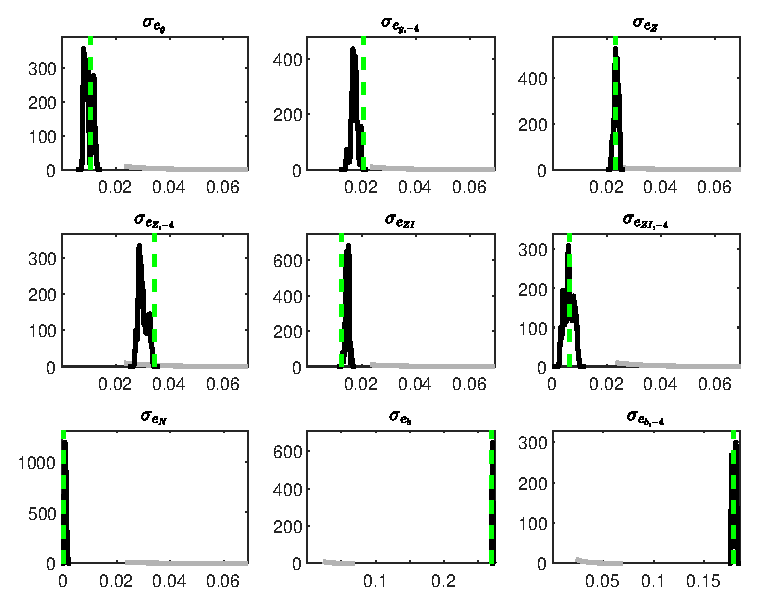
\includegraphics[width=0.80\textwidth]{RBC_sectoral/Output/RBC_sectoral_PriorsAndPosteriors1}
\caption{Priors and posteriors.}\label{Fig:PriorsAndPosteriors:1}
\end{figure}
 
\begin{figure}[H]
\centering
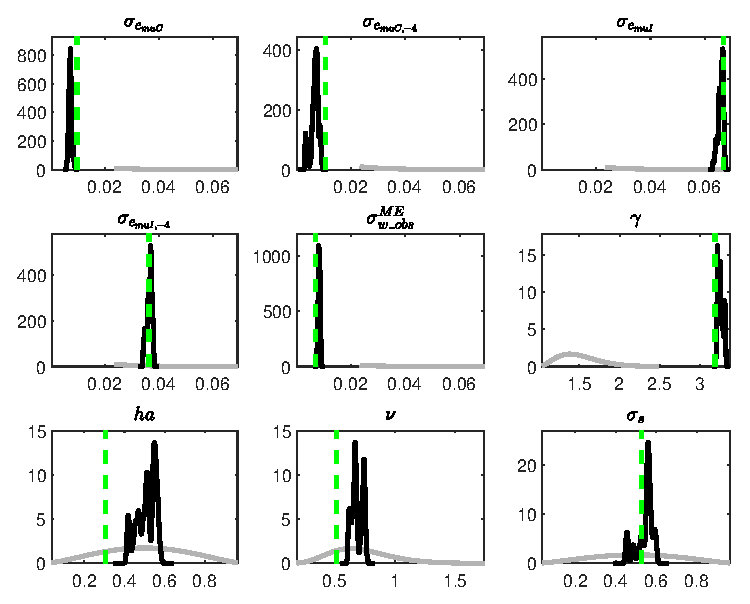
\includegraphics[width=0.80\textwidth]{RBC_sectoral/Output/RBC_sectoral_PriorsAndPosteriors2}
\caption{Priors and posteriors.}\label{Fig:PriorsAndPosteriors:2}
\end{figure}
 
\begin{figure}[H]
\centering
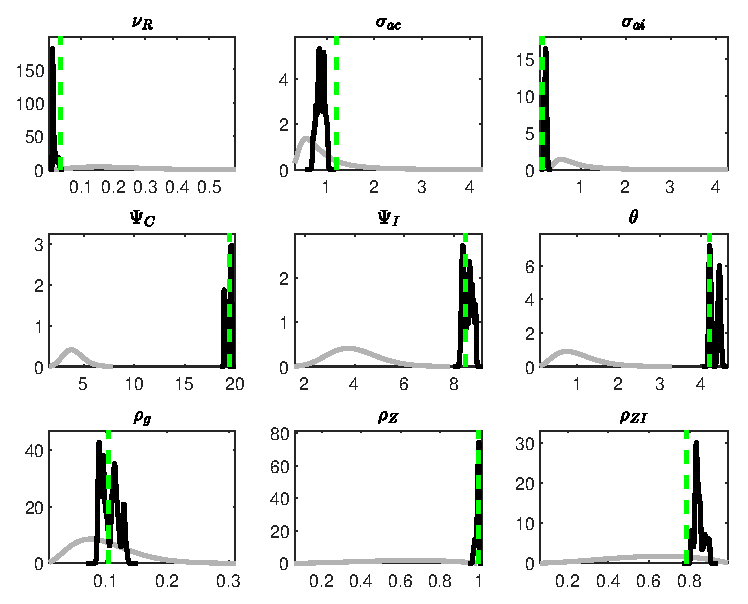
\includegraphics[width=0.80\textwidth]{RBC_sectoral/Output/RBC_sectoral_PriorsAndPosteriors3}
\caption{Priors and posteriors.}\label{Fig:PriorsAndPosteriors:3}
\end{figure}
 
\begin{figure}[H]
\centering
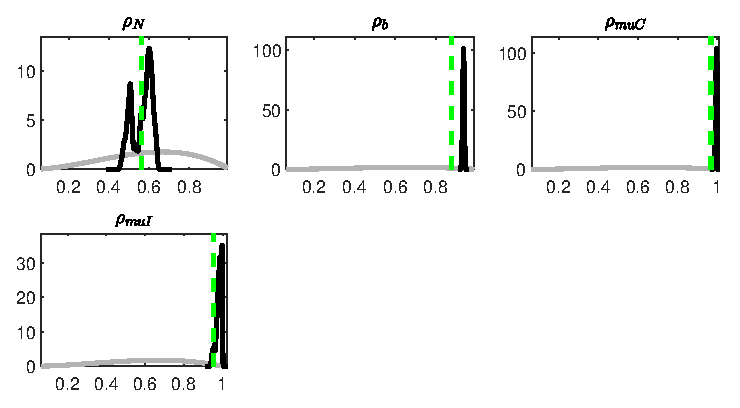
\includegraphics[width=0.80\textwidth]{RBC_sectoral/Output/RBC_sectoral_PriorsAndPosteriors4}
\caption{Priors and posteriors.}\label{Fig:PriorsAndPosteriors:4}
\end{figure}
 
% End of TeX file.
 
\include{RBC_sectoral/Output/RBC_sectoral_UnivariateDiagnostics} 
% TeX eps-loader file generated by mode_check.m (Dynare).
% 28-Mar-2024 17:50:39
 
\begin{figure}[H]
\centering 
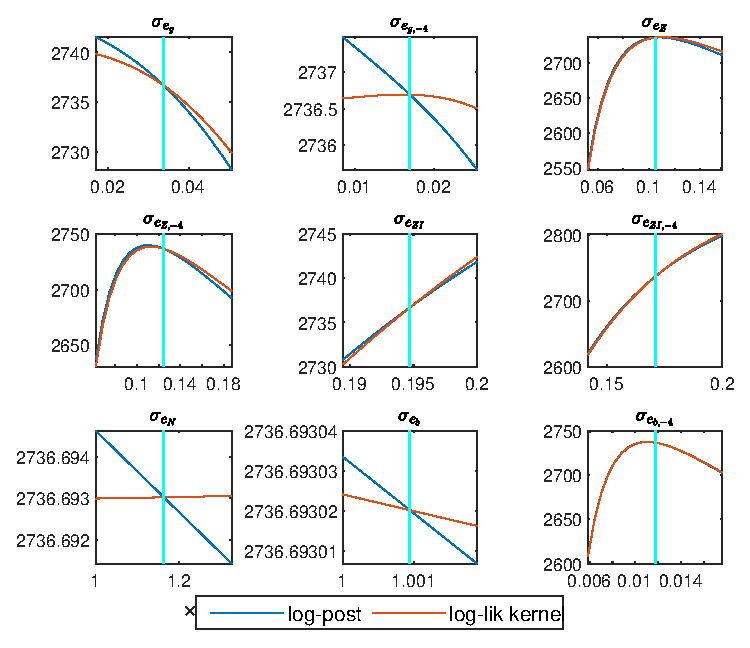
\includegraphics[width=0.80\textwidth]{RBC_sectoral/graphs/RBC_sectoral_CheckPlots1}
\caption{Check plots.}\label{Fig:CheckPlots:1}
\end{figure}
 
\begin{figure}[H]
\centering 
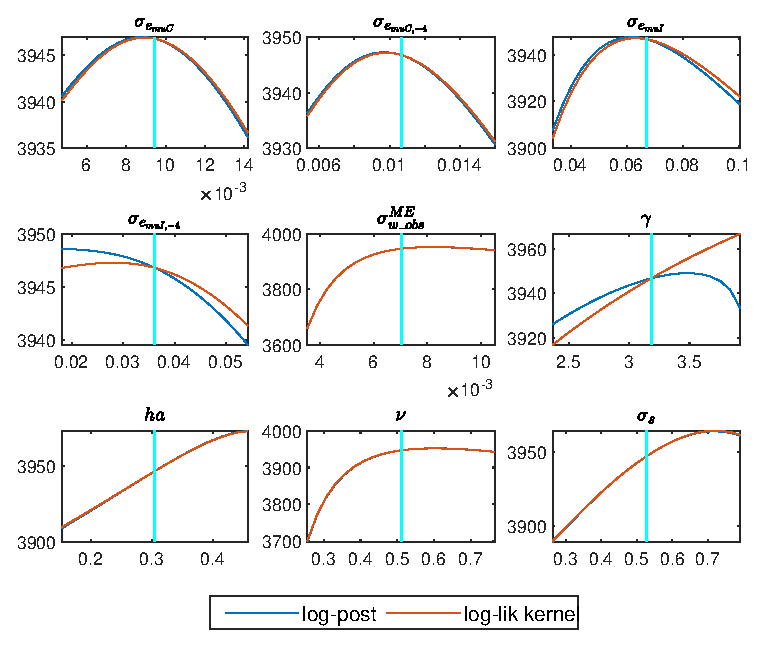
\includegraphics[width=0.80\textwidth]{RBC_sectoral/graphs/RBC_sectoral_CheckPlots2}
\caption{Check plots.}\label{Fig:CheckPlots:2}
\end{figure}
 
\begin{figure}[H]
\centering 
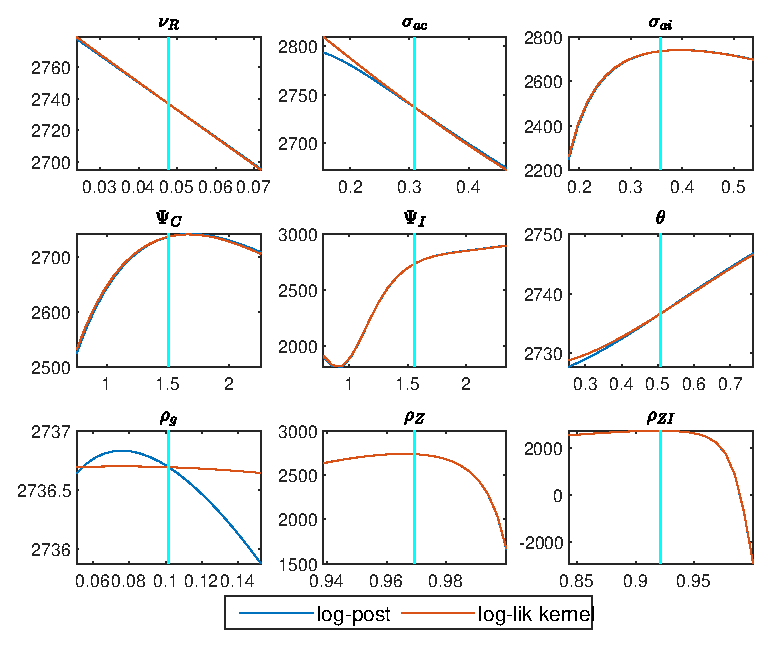
\includegraphics[width=0.80\textwidth]{RBC_sectoral/graphs/RBC_sectoral_CheckPlots3}
\caption{Check plots.}\label{Fig:CheckPlots:3}
\end{figure}
 
\begin{figure}[H]
\centering 
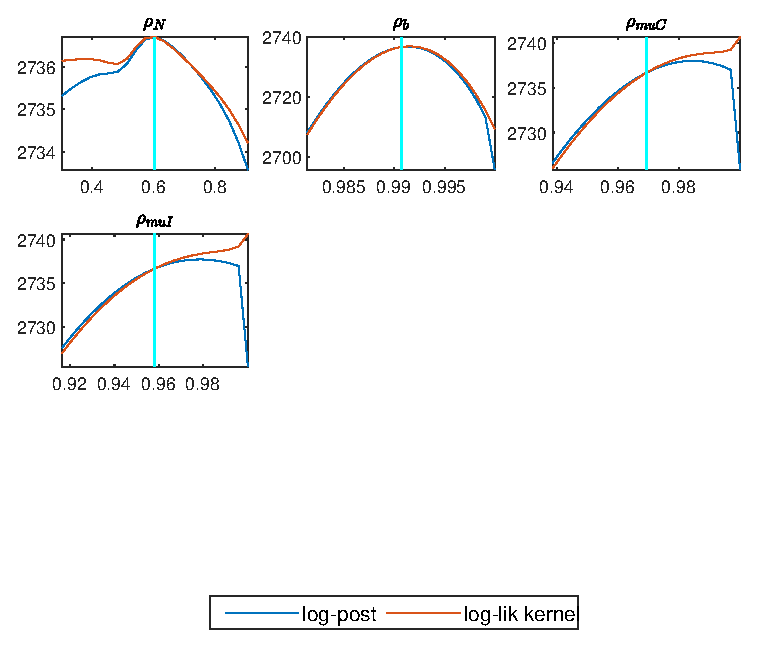
\includegraphics[width=0.80\textwidth]{RBC_sectoral/graphs/RBC_sectoral_CheckPlots4}
\caption{Check plots.}\label{Fig:CheckPlots:4}
\end{figure}
 
 
% TeX eps-loader file generated by dynare_estimation_1.m (Dynare).
% 28-Mar-2024 18:56:28
 
\begin{figure}[H]
\centering 
\includegraphics[width=0.80\textwidth]{RBC_sectoral/graphs/RBC_sectoral_HistoricalAndSmoothedVariables1}
\caption{Historical and smoothed variables.}\label{Fig:HistoricalAndSmoothedVariables:1}
\end{figure}


% End of TeX file.
 
% TeX eps-loader file generated by stoch_simul.m (Dynare).
% 28-Mar-2024 18:56:29
 
\begin{figure}[H]
\centering 
\includegraphics[width=0.80\textwidth]{RBC_sectoral/graphs/RBC_sectoral_IRF_e_g1}
\caption{Impulse response functions (orthogonalized shock to ${e_g}$).}\label{Fig:IRF:e_g:1}
\end{figure}
 
\begin{figure}[H]
\centering 
\includegraphics[width=0.80\textwidth]{RBC_sectoral/graphs/RBC_sectoral_IRF_e_g2}
\caption{Impulse response functions (orthogonalized shock to ${e_g}$).}\label{Fig:IRF:e_g:2}
\end{figure}
 
\begin{figure}[H]
\centering 
\includegraphics[width=0.80\textwidth]{RBC_sectoral/graphs/RBC_sectoral_IRF_e_g_news1}
\caption{Impulse response functions (orthogonalized shock to ${e_{g,-4}}$).}\label{Fig:IRF:e_g_news:1}
\end{figure}
 
\begin{figure}[H]
\centering 
\includegraphics[width=0.80\textwidth]{RBC_sectoral/graphs/RBC_sectoral_IRF_e_g_news2}
\caption{Impulse response functions (orthogonalized shock to ${e_{g,-4}}$).}\label{Fig:IRF:e_g_news:2}
\end{figure}
 
\begin{figure}[H]
\centering 
\includegraphics[width=0.80\textwidth]{RBC_sectoral/graphs/RBC_sectoral_IRF_e_Z1}
\caption{Impulse response functions (orthogonalized shock to ${e_Z}$).}\label{Fig:IRF:e_Z:1}
\end{figure}
 
\begin{figure}[H]
\centering 
\includegraphics[width=0.80\textwidth]{RBC_sectoral/graphs/RBC_sectoral_IRF_e_Z2}
\caption{Impulse response functions (orthogonalized shock to ${e_Z}$).}\label{Fig:IRF:e_Z:2}
\end{figure}
 
\begin{figure}[H]
\centering 
\includegraphics[width=0.80\textwidth]{RBC_sectoral/graphs/RBC_sectoral_IRF_e_Z_news1}
\caption{Impulse response functions (orthogonalized shock to ${e_{Z,-4}}$).}\label{Fig:IRF:e_Z_news:1}
\end{figure}
 
\begin{figure}[H]
\centering 
\includegraphics[width=0.80\textwidth]{RBC_sectoral/graphs/RBC_sectoral_IRF_e_Z_news2}
\caption{Impulse response functions (orthogonalized shock to ${e_{Z,-4}}$).}\label{Fig:IRF:e_Z_news:2}
\end{figure}
 
\begin{figure}[H]
\centering 
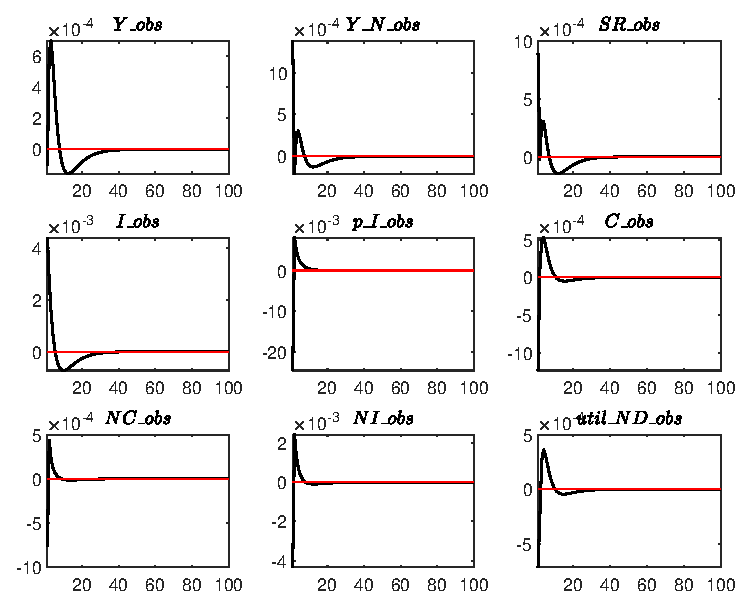
\includegraphics[width=0.80\textwidth]{RBC_sectoral/graphs/RBC_sectoral_IRF_e_ZI1}
\caption{Impulse response functions (orthogonalized shock to ${e_{ZI}}$).}\label{Fig:IRF:e_ZI:1}
\end{figure}
 
\begin{figure}[H]
\centering 
\includegraphics[width=0.80\textwidth]{RBC_sectoral/graphs/RBC_sectoral_IRF_e_ZI2}
\caption{Impulse response functions (orthogonalized shock to ${e_{ZI}}$).}\label{Fig:IRF:e_ZI:2}
\end{figure}
 
\begin{figure}[H]
\centering 
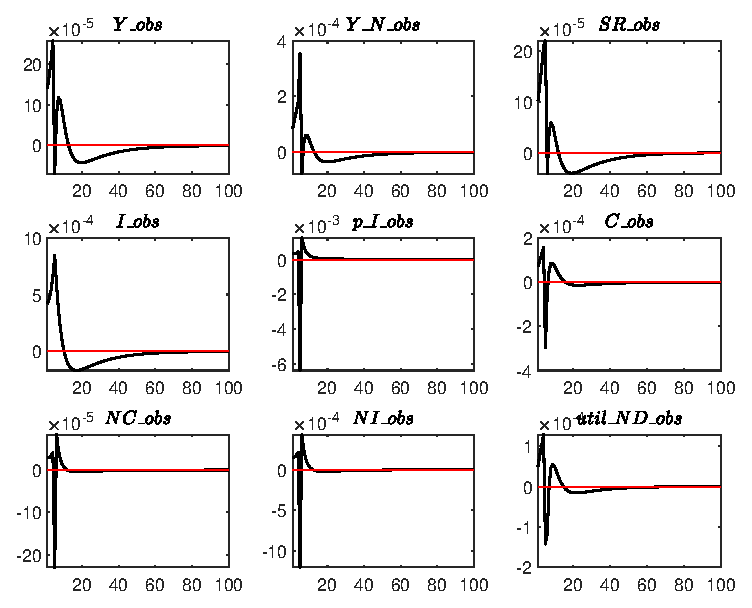
\includegraphics[width=0.80\textwidth]{RBC_sectoral/graphs/RBC_sectoral_IRF_e_ZI_news1}
\caption{Impulse response functions (orthogonalized shock to ${e_{ZI,-4}}$).}\label{Fig:IRF:e_ZI_news:1}
\end{figure}
 
\begin{figure}[H]
\centering 
\includegraphics[width=0.80\textwidth]{RBC_sectoral/graphs/RBC_sectoral_IRF_e_ZI_news2}
\caption{Impulse response functions (orthogonalized shock to ${e_{ZI,-4}}$).}\label{Fig:IRF:e_ZI_news:2}
\end{figure}
 
\begin{figure}[H]
\centering 
\includegraphics[width=0.80\textwidth]{RBC_sectoral/graphs/RBC_sectoral_IRF_e_N1}
\caption{Impulse response functions (orthogonalized shock to ${e_N}$).}\label{Fig:IRF:e_N:1}
\end{figure}
 
\begin{figure}[H]
\centering 
\includegraphics[width=0.80\textwidth]{RBC_sectoral/graphs/RBC_sectoral_IRF_e_N2}
\caption{Impulse response functions (orthogonalized shock to ${e_N}$).}\label{Fig:IRF:e_N:2}
\end{figure}
 
\begin{figure}[H]
\centering 
\includegraphics[width=0.80\textwidth]{RBC_sectoral/graphs/RBC_sectoral_IRF_e_b1}
\caption{Impulse response functions (orthogonalized shock to ${e_b}$).}\label{Fig:IRF:e_b:1}
\end{figure}
 
\begin{figure}[H]
\centering 
\includegraphics[width=0.80\textwidth]{RBC_sectoral/graphs/RBC_sectoral_IRF_e_b2}
\caption{Impulse response functions (orthogonalized shock to ${e_b}$).}\label{Fig:IRF:e_b:2}
\end{figure}
 
\begin{figure}[H]
\centering 
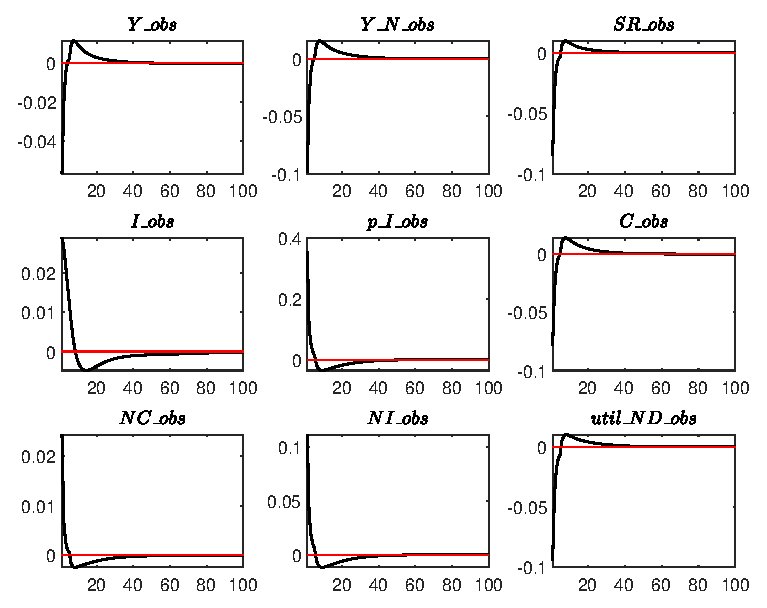
\includegraphics[width=0.80\textwidth]{RBC_sectoral/graphs/RBC_sectoral_IRF_e_b_news1}
\caption{Impulse response functions (orthogonalized shock to ${e_{b,-4}}$).}\label{Fig:IRF:e_b_news:1}
\end{figure}
 
\begin{figure}[H]
\centering 
\includegraphics[width=0.80\textwidth]{RBC_sectoral/graphs/RBC_sectoral_IRF_e_b_news2}
\caption{Impulse response functions (orthogonalized shock to ${e_{b,-4}}$).}\label{Fig:IRF:e_b_news:2}
\end{figure}
 
\begin{figure}[H]
\centering 
\includegraphics[width=0.80\textwidth]{RBC_sectoral/graphs/RBC_sectoral_IRF_e_muC1}
\caption{Impulse response functions (orthogonalized shock to ${e_{muC}}$).}\label{Fig:IRF:e_muC:1}
\end{figure}
 
\begin{figure}[H]
\centering 
\includegraphics[width=0.80\textwidth]{RBC_sectoral/graphs/RBC_sectoral_IRF_e_muC2}
\caption{Impulse response functions (orthogonalized shock to ${e_{muC}}$).}\label{Fig:IRF:e_muC:2}
\end{figure}
 
\begin{figure}[H]
\centering 
\includegraphics[width=0.80\textwidth]{RBC_sectoral/graphs/RBC_sectoral_IRF_e_muC_news1}
\caption{Impulse response functions (orthogonalized shock to ${e_{muC,-4}}$).}\label{Fig:IRF:e_muC_news:1}
\end{figure}
 
\begin{figure}[H]
\centering 
\includegraphics[width=0.80\textwidth]{RBC_sectoral/graphs/RBC_sectoral_IRF_e_muC_news2}
\caption{Impulse response functions (orthogonalized shock to ${e_{muC,-4}}$).}\label{Fig:IRF:e_muC_news:2}
\end{figure}
 
\begin{figure}[H]
\centering 
\includegraphics[width=0.80\textwidth]{RBC_sectoral/graphs/RBC_sectoral_IRF_e_muI1}
\caption{Impulse response functions (orthogonalized shock to ${e_{muI}}$).}\label{Fig:IRF:e_muI:1}
\end{figure}
 
\begin{figure}[H]
\centering 
\includegraphics[width=0.80\textwidth]{RBC_sectoral/graphs/RBC_sectoral_IRF_e_muI2}
\caption{Impulse response functions (orthogonalized shock to ${e_{muI}}$).}\label{Fig:IRF:e_muI:2}
\end{figure}
 
\begin{figure}[H]
\centering 
\includegraphics[width=0.80\textwidth]{RBC_sectoral/graphs/RBC_sectoral_IRF_e_muI_news1}
\caption{Impulse response functions (orthogonalized shock to ${e_{muI,-4}}$).}\label{Fig:IRF:e_muI_news:1}
\end{figure}
 
\begin{figure}[H]
\centering 
\includegraphics[width=0.80\textwidth]{RBC_sectoral/graphs/RBC_sectoral_IRF_e_muI_news2}
\caption{Impulse response functions (orthogonalized shock to ${e_{muI,-4}}$).}\label{Fig:IRF:e_muI_news:2}
\end{figure}
 
 
% End Of TeX file. 
 
\include{RBC_sectoral/graphs/RBC_sectoral_Priors} 
% TeX eps-loader file generated by dynare_estimation_1.m (Dynare).
% 28-Mar-2024 18:56:28
 
\begin{figure}[H]
\centering 
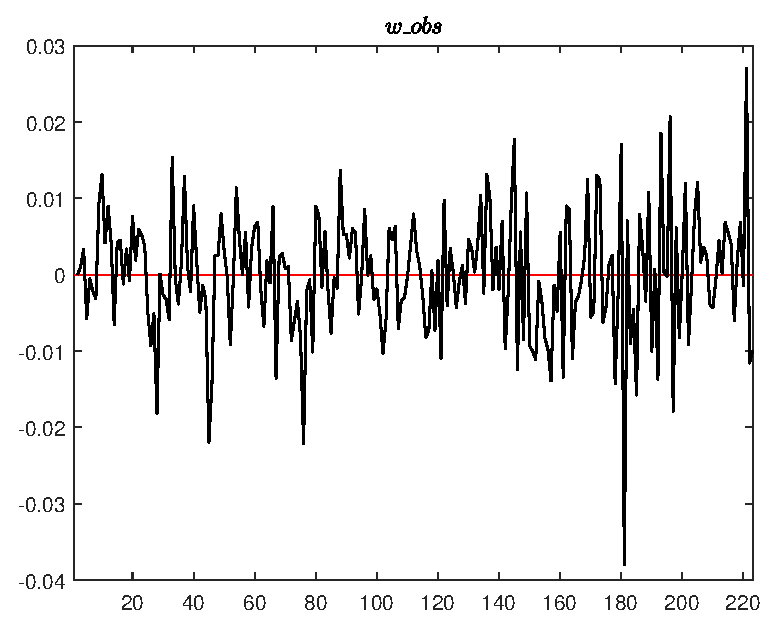
\includegraphics[width=0.80\textwidth]{RBC_sectoral/graphs/RBC_sectoral_SmoothedObservationErrors1}
\caption{Smoothed observation errors.}\label{Fig:SmoothedObservationErrors:1}
\end{figure}


% End of TeX file.
 
% TeX eps-loader file generated by dynare_estimation_1.m (Dynare).
% 28-Mar-2024 18:56:27
 
\begin{figure}[H]
\centering 
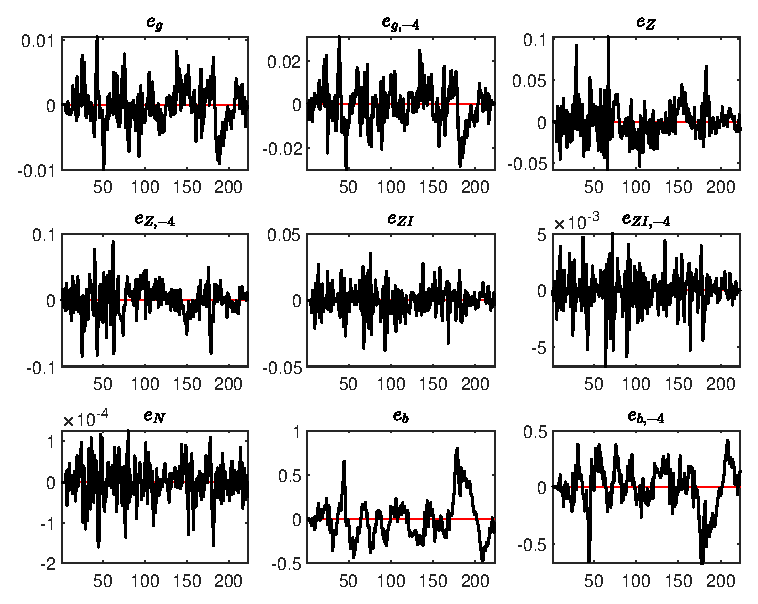
\includegraphics[width=0.80\textwidth]{RBC_sectoral/graphs/RBC_sectoral_SmoothedShocks1}
\caption{Smoothed shocks.}\label{Fig:SmoothedShocks:1}
\end{figure}

\begin{figure}[H]
\centering 
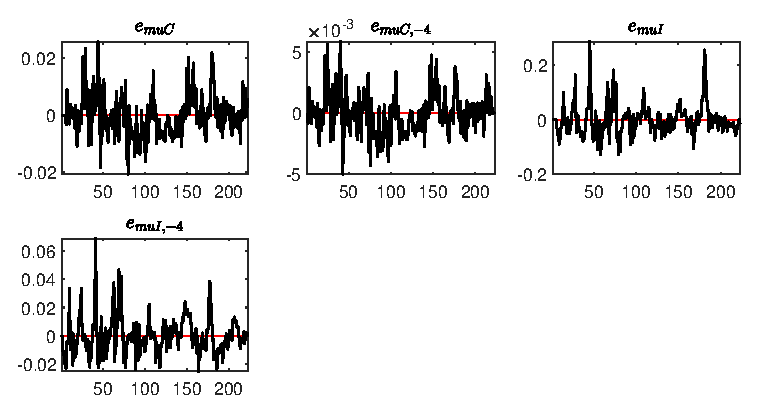
\includegraphics[width=0.80\textwidth]{RBC_sectoral/graphs/RBC_sectoral_SmoothedShocks2}
\caption{Smoothed shocks.}\label{Fig:SmoothedShocks:2}
\end{figure}


% End of TeX file.
 
\end{document} 
